\section{Hiérarchie mémoire} \label{sec:hierarchie}
%%%%%%%%%%%%%%%%%%%%%%%%%%%%%%%%%%%%%%%%%%%%%%%%%%%%%%%%%%%%%%%%%%%

%\begin{fancyquotes}
%Idéalement, on souhaiterait disposer d'une capacité de mémoire indéfiniment grande, de sorte qu'un agrégat particulier de 40 chiffres binaires, ou mot (cf. 2.3), soit immédiatement disponible, c'est-à-dire dans un temps légèrement ou considérablement plus court que le temps de fonctionnement d'un multiplicateur électronique rapide. On peut supposer que cela est pratique au niveau d'environ 100 m sec. Par conséquent, le temps de disponibilité d'un mot dans la mémoire doit être de 5 à 50 ms. Il est également souhaitable que les mots puissent être remplacés par de nouveaux mots à peu près au même rythme. Il ne semble pas physiquement possible d'atteindre une telle capacité. Nous sommes donc obligés de reconnaître la possibilité de construire une hiérarchie de mémoires, chacune d'entre elles ayant une plus grande capacité que la précédente mais moins rapidement accessible.\\
%Traduit de \cite{burks1946preliminary}.

%\end{fancyquotes}


  

Dans la partie précédente sont présentées les principales améliorations dont la microarchitecture a pu  bénéficier. Cette partie s'intéressait principalement à l'exécution des instructions. Pour être exécutées, ces instructions ont besoin de données stockées en mémoire. Ainsi, pour apprécier la performance totale du processeur, cette partie s'intéresse à la partie mémoire. 
La \autoref{sec:memory} présente la différence d'évolution entre les processeurs et la mémoire. Cette introduction permet de motiver la nécessité de construire une hiérarchie mémoire présentée dans la \autoref{sec:hierarchie_true}. Enfin, la \autoref{sec:cache} présente plus précisément les mémoires caches.


%%%%%%%%%%%%%%%%%%%%%%%%%%%%%%%%%%%%%%%%%%%%%%%%%%%%%%%%%%%%%%%%%%%
%%%%%%%%%%%%%%%%%%%%%%%%%%%%%%%%%%%%%%%%%%%%%%%%%%%%%%%%%%%%%%%%%%%
\subsection{Mémoire principale} \label{sec:memory}
%%%%%%%%%%%%%%%%%%%%%%%%%%%%%%%%%%%%%%%%%%%%%%%%%%%%%%%%%%%%%%%%%%%
%%%%%%%%%%%%%%%%%%%%%%%%%%%%%%%%%%%%%%%%%%%%%%%%%%%%%%%%%%%%%%%%%%%

Pour leur exécution, les processeurs doivent accéder aux instructions et aux données stockées en mémoire. Celles-ci sont principalement construites à partir de mémoire RAM (voir \autoref{sec:ram}). Ces mémoires, élaborées à partir de transistors, ont pu bénéficier des mêmes évolutions technologiques que les processeurs (voir \autoref{sec:moore}). Il est cependant connu de tous que l'écart des performances entre ces deux modules s'est agrandi année après année. 


%CONSTAT
\subsubsection{Performance de la mémoire et des processeurs}
%%%%%%%%%%%%%

À cause de la forte évolution du processeur, l'écart avec la performance des mémoires s'est creusé au fil des années (voir \autoref{pic:cpuvsmemory}). Le graphique utilise une échelle logarithmique, l'écart de performance entre les deux s’agrandit exponentiellement. La performance des processeurs a évolué de 70\% chaque année quand la latence mémoire n’est réduite que de 7\%.
L’augmentation du nombre de coeurs, toujours plus puissant (fréquence, pipeline, opérations vectorielles), se partageant un bus mémoire dont les performances évoluent lentement, implique une baisse de bande passante disponible par coeur. À l’inverse des besoins des applications, la bande passante par coeur diminue(voir \autoref{pic_cpu_bw_per_core}). 
 

 \begin{figure}
    \center
    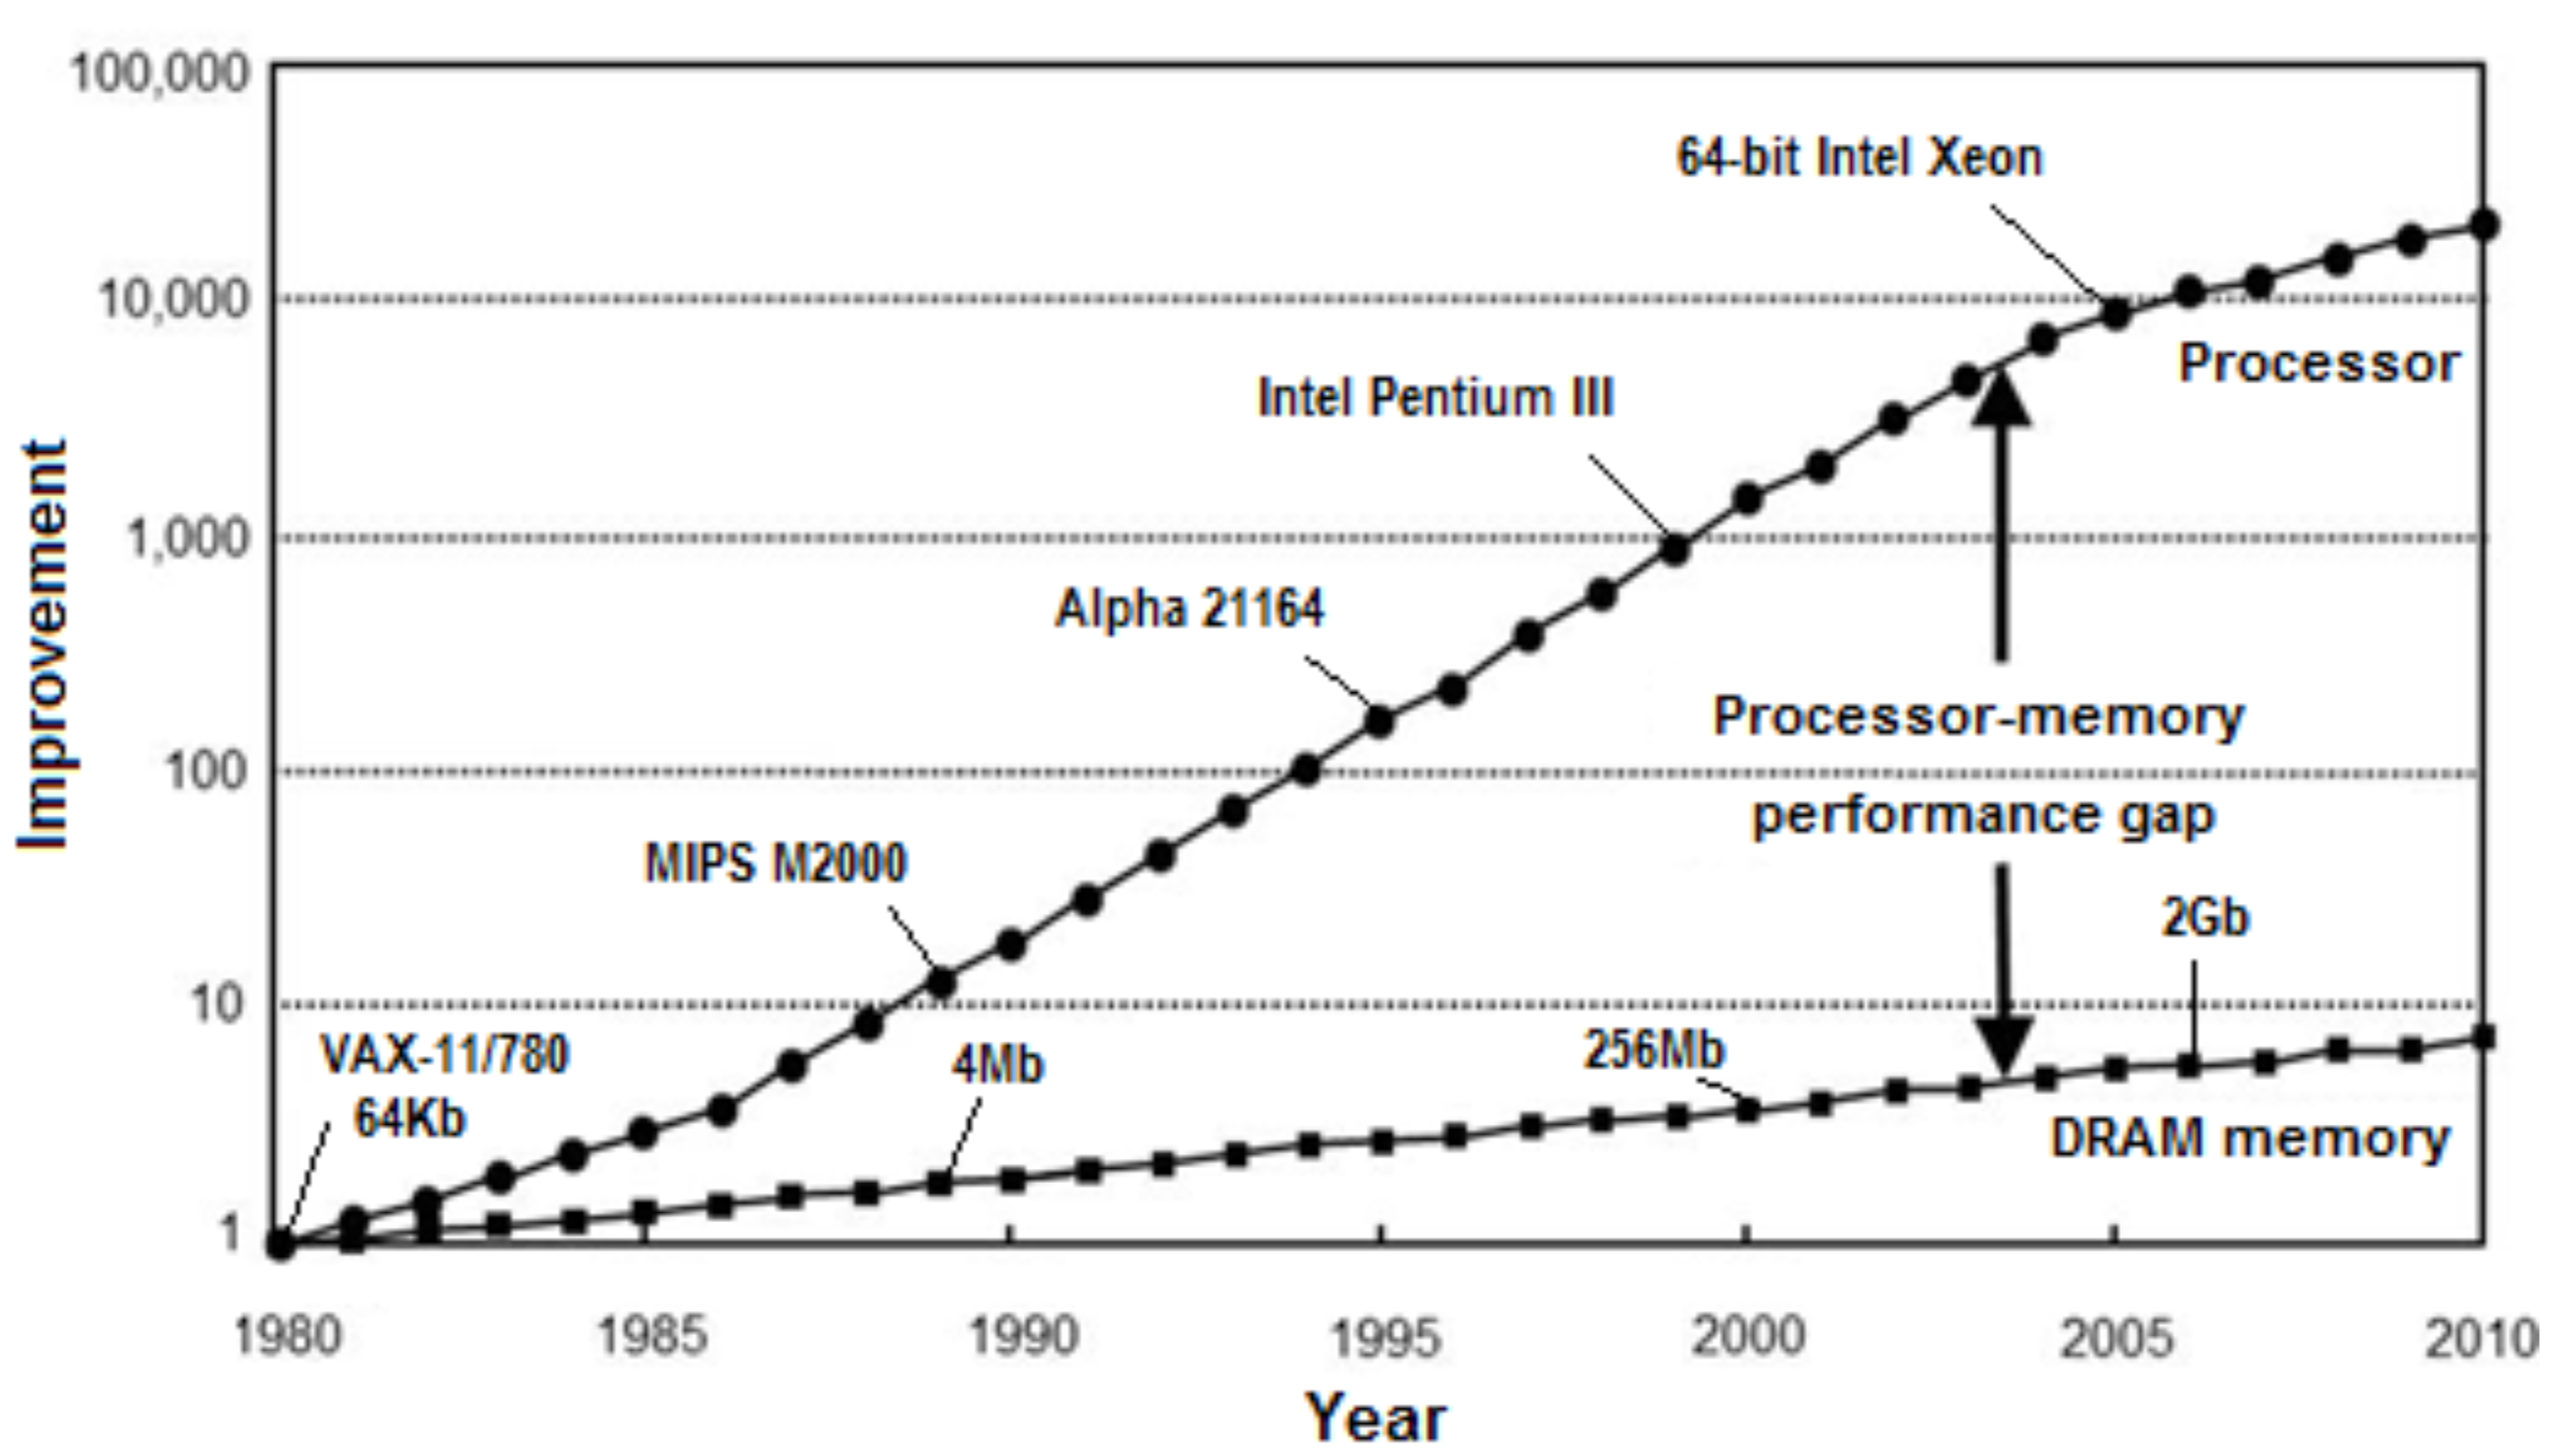
\includegraphics[width=8cm]{images/cpu_cpu_vs_memory.png}
    \caption{\label{pic:cpuvsmemory} Progression de la performance des processeurs et des mémoires. La performance de plusieurs générations de processeurs a été mesurée à l'aide du benchmark SPECint \cite{Efnusheva2017ASO}. La performance des mémoires est la mesure des latences d’accès mémoire (CAS et RAS) des mémoires DRAM.}
\end{figure}



\begin{figure}
    \center
    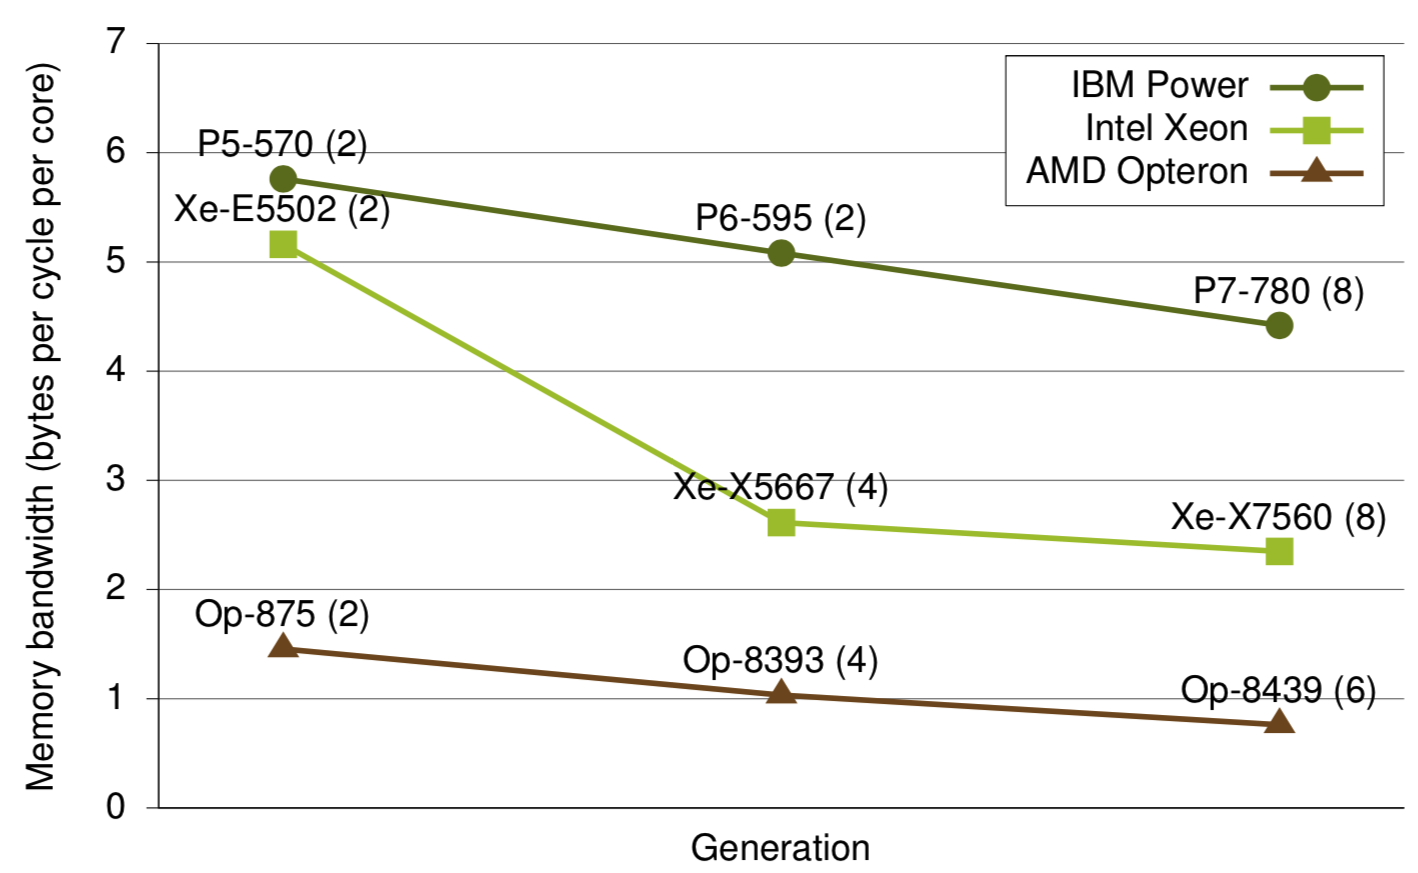
\includegraphics[width=8cm]{images/cpu_bw_per_core.png}
    \caption{Évolution de la bande passante bande passante par cycle d'horloge par coeur  \cite{CacheInjection}. L'évolution du nombre de coeurs et de leur fréquence n'est pas compensée par l'évolution de la performance du système mémoire.
    \label{pic_cpu_bw_per_core}}
\end{figure}



% EXPLICATION
\subsubsection{Le mur de la mémoire}\label{sec:memory_wall_gap}
L'écart croissant entre les performances de la mémoire et des processeurs est souvent appelé \textit{mur de la mémoire} (\textit{memory wall}). Cette expression été déjà utilisée en 1995 \cite{Wulf1995} dans le papier \textit{Hitting the Memory Wall: Implications of the Obvious}. Plusieurs raisons peuvent expliquer cet écart de performance.


\paragraph{Économiques.}
L'économie du marché des mémoires est une première explication. Le prix par gigaoctet diminue avec la densité des mémoires. Les fabricants d'ordinateurs et de téléphones souhaitent avoir des mémoires de plus grande capacité dans des espaces restreints avec des contraintes énergétiques. La SRAM, moins dense et plus consommatrice est ainsi passée en second plan. Les différentes évolutions de ces deux technologies mémoires sont résumées dans le \autoref{tab_ddr}.  La mémoire DRAM à vu ses performances évoluer d'un facteur 10 depuis les premières versions de \textit{SDRAM} dans les années 90. Le passage de la SDRAM à la \textit{Double Data Rate} (DRAM) permet d'envoyer deux données par signal d'horloge. Les principales évolutions des performances de ces technologies sont résumées dans le \autoref{tab_ddr}. 

\begin{table}[]
\centering
\resizebox{\textwidth}{!}{%
\begin{tabular}{@{}|l|c|c|c|c|c|@{}}
\toprule
\rowcolor[HTML]{EFEFEF} 
\textbf{DDR Standard} & \multicolumn{1}{l|}{\cellcolor[HTML]{EFEFEF}\textbf{Débit (MT/s)}}     & \multicolumn{1}{l|}{\cellcolor[HTML]{EFEFEF}\textbf{Densité (MiB)}} & \multicolumn{1}{l|}{\cellcolor[HTML]{EFEFEF}\textbf{Bande passante (GB/s)}} & \multicolumn{1}{l|}{\cellcolor[HTML]{EFEFEF}\textbf{Latence (ns)}}           & \multicolumn{1}{l|}{\cellcolor[HTML]{EFEFEF}\textbf{Tension (V)}} \\ \midrule
SDRAM    &      100-166         & 1          & 0.8-1.3        & 90-75            & 3.3       \\ \midrule
DDR      &      133-200         & 128         & 1-3.1        & 36-30            & 2.5       \\ \midrule
DDR2     &      400-1066        & 256         & 3.2-8.3        & 37.5-14.06       & 1.8       \\ \midrule
DDR3     &      1066-3300       & 1024       & 8.3-25.8       & 19.69-11.82      & 1.5       \\ \midrule
DDR4     &      1600-4800       & 4096       & 12.5-37.5        & 19.38-9.38       & 1.2       \\ \bottomrule
\end{tabular}%
}
\caption[Évolution des technologies de mémoire DRAM]{Les évolutions des technologies mémoires DDR ont permis d'améliorer les vitesses de transferts d'un facteur dix en divisant par trois leur consommation électrique\protect\footnotemark. Pour chaque standard DDR, les débits et la latence sont donnés pour deux fréquences différentes. La latence mesure le temps nécessaire pour transférer  8 mots (soit une ligne de cache). Cette mesure est plus précise, car les versions les plus récentes de DDR lisent plusieurs mots à la fois dans une mémoire tampon, et profite donc de la localité spatiale.}
\label{tab_ddr}
\end{table}
\footnotetext{source: \url{https://www.transcend-info.com/Support/FAQ-296}, \url{https://promotions.newegg.com/crucial/15-2725/index.html?icid=318028}, \url{https://en.wikipedia.org/wiki/CAS_latency} \url{https://www.crucial.com/usa/en/memory-performance-speed-latency}}


\paragraph{Technologiques.} Le gain de transistors assuré par la loi de Moore a donc été utilisé pour construire des mémoires plus denses et donc de plus grande capacité. Cependant, l’industrie des microprocesseurs a profité de ces transistors pour construire des processeurs plus performants tandis que l’industrie des mémoires en a profité pour créer des mémoires de plus grande capacité. Le bus mémoire reliant la mémoire au processeur limite lui la bande passante mémoire. La raison de sa faible évolution est que la construction d'un bus plus performant nécessite d'utiliser plus de broches. Les bus actuels utilisent déjà presque $NbPinParChannel*NbChannel/nombrePinPerProcessor$\% (\textbf{à faire} des broches disponibles.\\

D'un côté, les processeurs sont plus rapides et plus puissants. D'un autre côté, les mémoires voient leur capacité de stockage augmenter. Ainsi, les mémoires doivent transférer plus de données et plus rapidement au processeur. Ce problème est d'autant plus exacerbé par l'architecture des processeurs. L’architecture Von Neumann (voir \autoref{sec:von}) implémente une microarchitecture qui sépare la partie exécution de la partie mémoire.
Le processeur a besoin des instructions et des données stockées dans la mémoire ce qui implique de nombreuses communications entre ces deux parties. Le bus mémoire devient un \textit{goulot d'étranglement} pour les performances (ou \textit{bottleneck}). Il a ainsi été nommé d'après l'architecte: le \textit{bottleneck Von Neumann}.




% SOLUTION
\subsubsection{Solutions}
La latence mémoire est le temps écoulé entre l’initiation d’un transfert mémoire et l'arrivée de la donnée sur le processeur. Bien qu'elle puisse être considérée comme constante, il est possible de réduire la latence du point de vue du processeur en initiant les transferts avant qu'ils ne commencent.  Lest architectures ont reçues plusieurs améliorations matérielles et logicielles pour \textit{réduire} ou \textit{tolérer} les latences mémoires \cite{Efnusheva2017ASO}.



\paragraph{Améliorer la latence mémoire.} 
La prélecture mémoire \cite{baer1991effective, mowry1991tolerating} ou \textit{memory prefteching}  a pour objectif de prédire les futurs accès mémoire pour réduire ou supprimer la latence lors d'un accès mémoire. La prélecture peut être réalisée par le système d'exploitation ou par le compilateur en se basant sur des motifs d'accès pour anticiper les prochains appels mémoires. Elle peut aussi être implémentée manuellement dans l'application en utilisant des instructions spécifiques ou en anticipant les accès. Cette technique, utilisée parfaitement, peut supprimer toutes les latences impactant une application. Cependant, la caractéristique principale du bus mémoire qui réduit les performances des applications est la bande passante.

\paragraph{Tolérer les latences.}
La deuxième solution aux latences mémoires est de les tolérer \cite{Bakshi2000}. Les techniques de tolérance aux latences permettent au processeur de continuer d’exécuter des instructions durant latente d’une donnée: l’exécution dans le désordre (\autoref{sec:out_of_order}) ou la prédiction de branchement (\autoref{sec:branch_predictor}).\\

Si les latences peuvent être réduites ou tolérer, la bande passante du bus mémoire contraint elle aussi la performance des applications. La principale réponse à ce challenge est l’implémentation d’une hiérarchie de mémoire plus ou moins rapide en fonction de leur proximité avec le processeur. 


%%%%%%%%%%%%%%%%%%%%%%%%%%%%%%%%%%%%%%%%%%%%%%%%%%%%%%%%%%%%%%%%%%%
\subsection{Compromis entre le coût, la performance et la capacité } \label{sec:hierarchie_true}
%%%%%%%%%%%%%%%%%%%%%%%%%%%%%%%%%%%%%%%%%%%%%%%%%%%%%%%%%%%%%%%%%%%

La réponse naïve au problème du \textit{memory wall} est de construire de grandes mémoires à partir de SRAM, très performantes et qui consomment peu d'énergie. Cependant, des contraintes économiques et techniques sont à prendre en compte et rendent impossible cette solution. La mémoire SRAM est très chère à produire et nécessite l'utilisation de six transistors pour fonctionner, empêchant la construction de modules denses. 

Dans le \autoref{pic_cpu_memory_comparison}, on remarque que trois caractéristiques sont liées entres elles. Au plus la latence d'accès à la mémoire est petite, au plus son prix est élevé. Plus la capacité d'une mémoire au plus son prix par bit est réduit. Plus la capacité est élevée plus la latence d'accès est grande.
L'objectif des constructeurs d'ordinateur est de proposer une mémoire à la fois très rapide à un prix le plus faible possible. Ce qui n'est malheureusement le cas d'aucune des technologies existantes. Pour atteindre cet objectif, la solution imaginée par les architectes est l'utilisation de différents tailles et types de mémoires constituant une \textit{hiérarchie de mémoires}.


\begin{figure}
    \center
    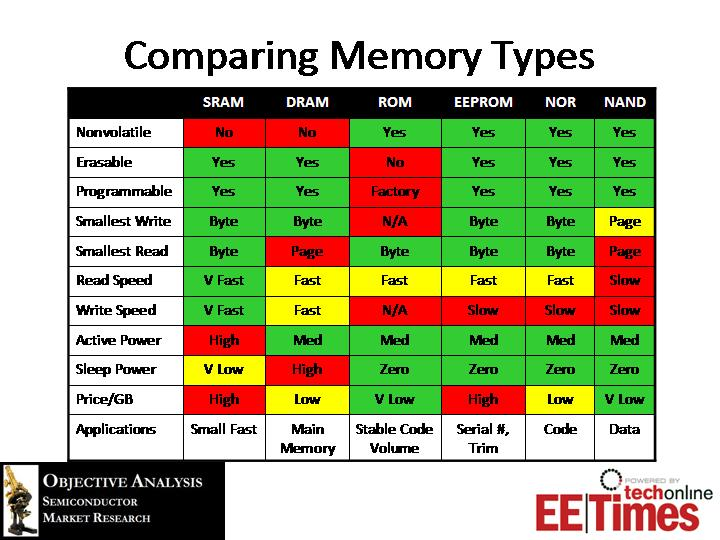
\includegraphics[width=10cm]{images/cpu_memory_comparison.jpg}
    \caption{\label{pic_cpu_memory_comparison} Comparaison des caratéristiques de différents types de mémoires.\textbf{todo:} faire un tableau avec des valeurs récentes et les prix. }
\end{figure}



La hiérarchie mémoire est la réponse d'un compromis entre le coût, la performance et la capacité de stockage pour la construction de la mémoire d'un processeur. Comme aucune des mémoires ne répond à ces trois facteurs à la fois, la solution est de ne pas se restreindre à  une seule technologie et d'utiliser des modules de taille différente (voir \autoref{pic_cpu_memory_hierarchy}). Le compromis réalisé par la hiérarchie mémoire permet ainsi de: réduire le coût par bit stocké, augmenter la capacité de la mémoire et améliorer le temps d'accès aux données. 

La solution est de placer au plus proche du processeur des mémoires très rapides pouvant répondre instantanément aux accès mémoire. Au plus on s'éloigne des unités de calcul, au plus la latence d'accès aux modules mémoires augmente, mais au plus leur prix diminue rendant possible l'utilisation de module de plus grande capacité. Lorsque le processeur souhaite accéder à une donnée, il vérifie qu'elle se trouve dans son premier niveau de mémoire et, si ce n'est pas le cas, remonte la hiérarchie jusqu'à la trouver. La performance des applications varie fortement si les données nécessaires sont présentes ou non dans les mémoires proches du processeur. L'apport d'un gain de performance de la hiérarchie réside dans le fait que la donnée accédée doit se trouver le plus souvent possible dans les zones mémoires les plus proches du processeur.


\begin{figure}
    \center
    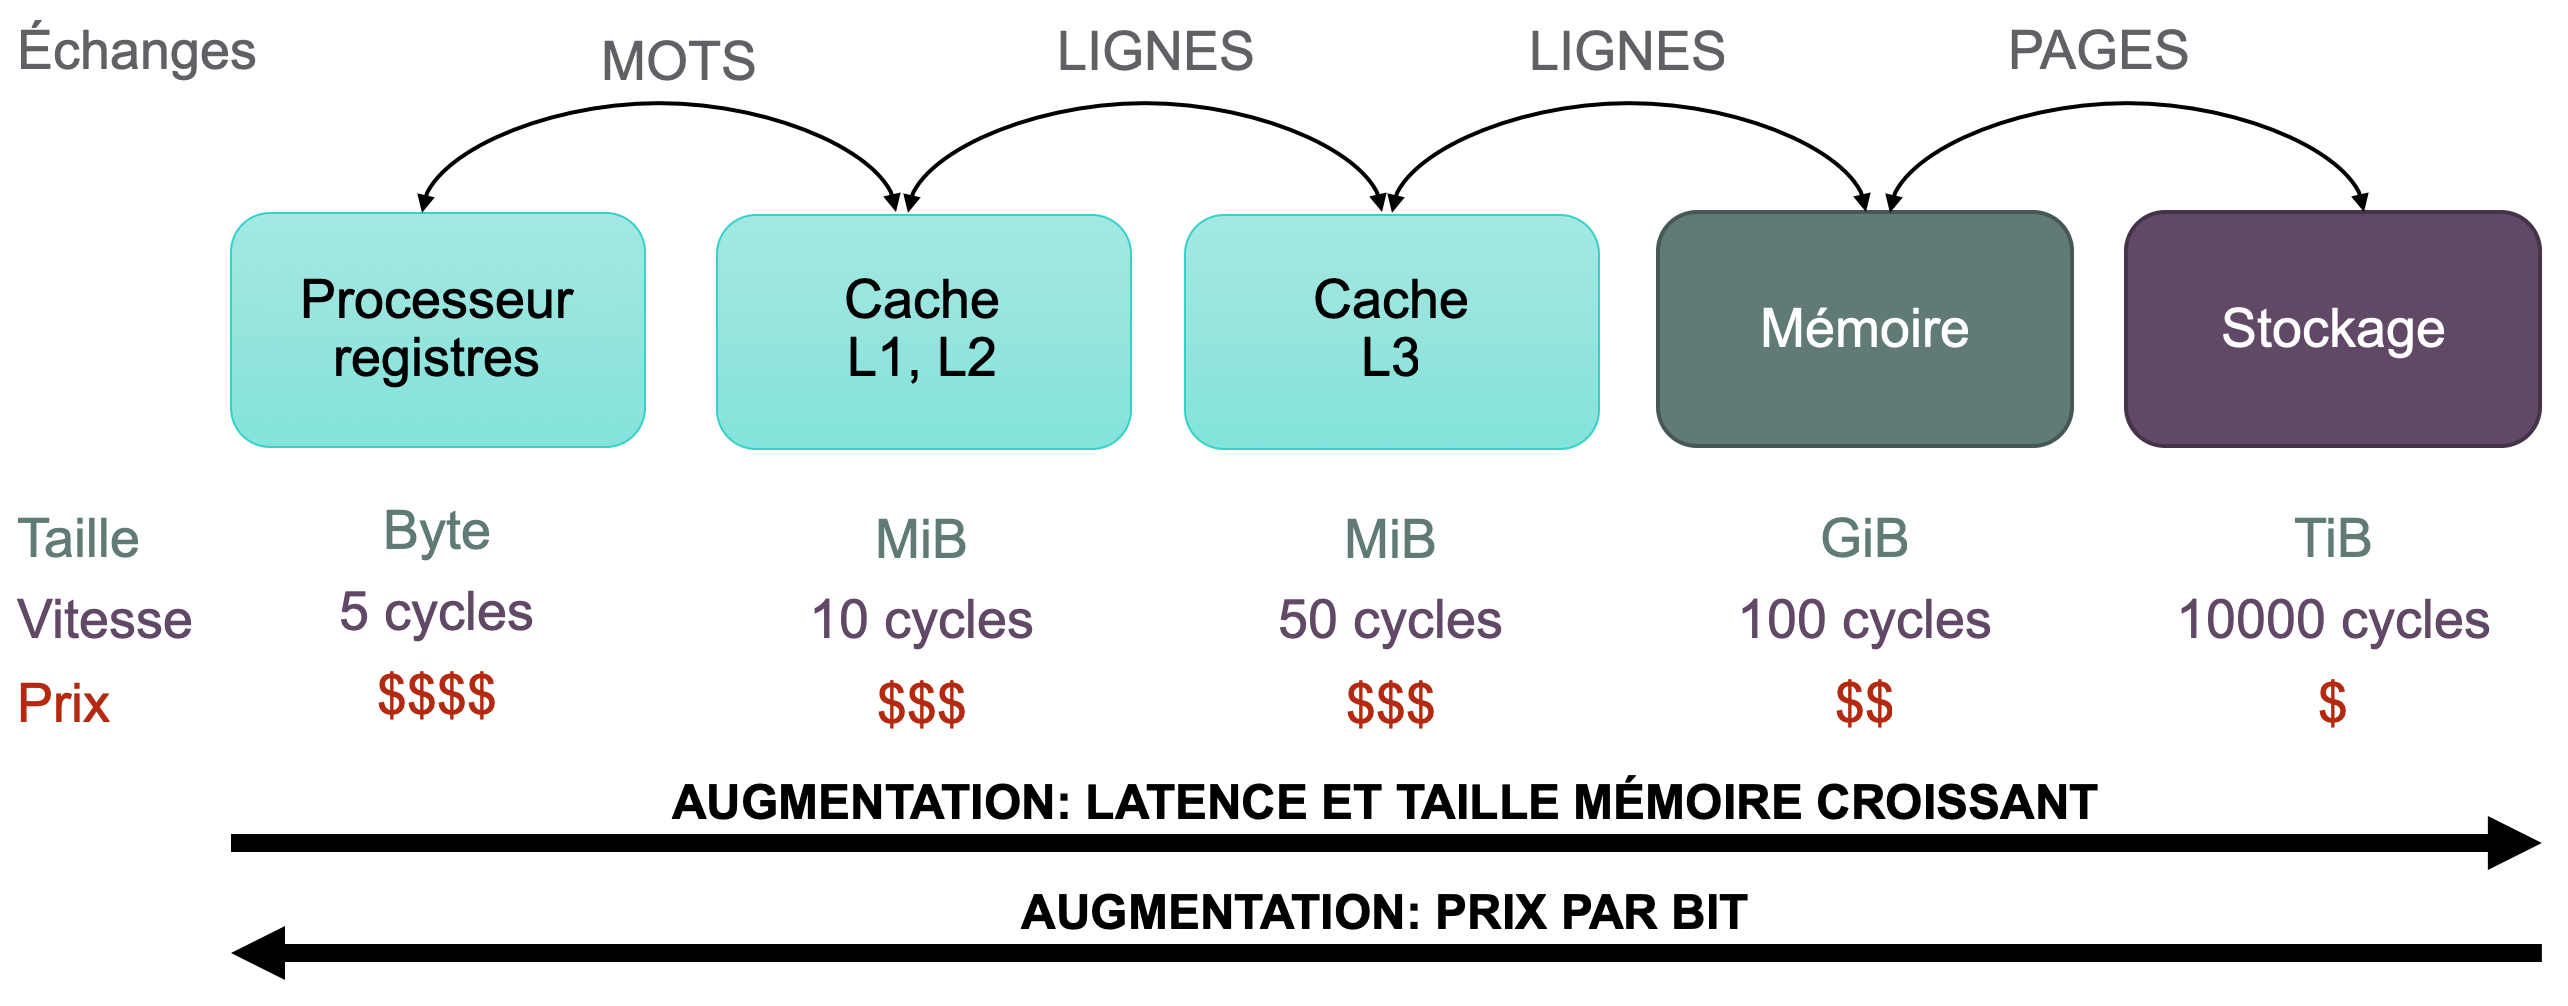
\includegraphics[width=10cm]{images/cpu_memory_hierarchy.png}
    \caption{\label{pic_cpu_memory_hierarchy} Hiérarchie mémoire}
\end{figure}

La \autoref{pic_cpu_memory_hierarchy} présente les principaux modules d'une hiérarchie mémoire d'un processeur moderne:
\begin{enumerate}
    
    \item Les registres: ils sont situés au plus proche des unités de calculs. Pour permettre un accès rapide, 1 cycle, ils sont réalisés en SRAM. On compte une centaine de registres sur les processeurs récents. Leur taille est variable en fonction des instructions exécutables par les unités logiques arithmétiques. Par exemple, un processeur pouvant exécuter des instructions vectorielles AVX-512, possède des registres de 512 bits (registre \textit{ZMM}). Il existe différents types de registres, certains sont utilisés pour stocker des données et des résultats intermédiaires, tandis que d'autres ont une signification précise. Le registre de pointeurs de piles stocke l'adresse de la première adresse mémoire responsable de l'instruction actuellement exécutée et permet de réaliser des appels et des retours de fonctions. Les registres des drapeaux (Flag Register) stockent des informations nécessaires à l'exécution d'instructions. Par exemple, lorsqu'une retenue est générée par un calcul, ou qu'un branchement conditionnel a été évalué à vrai. Les processeurs récents dupliquent certains registres pour pouvoir utiliser des techniques de renommage \cite{moudgill1993register} et d'exécution spéculative \cite{chou2004efficient}.

    \item Les caches ou \textit{antémémoire} sont des modules de mémoire généralement en SRAM à très faible latence d'accès (quelques cycles). Ces mémoires étant très chères, elles ne peuvent pas être construites en grande quantité. La performance d'une application dépendra fortement de la présence ou non des données nécessaires dans ces mémoires. Ce principe est connu sous le nom de concept de \textit{localité}, présenté dans la \autoref{sec:locality}. Les caches sont présentés plus précisément dans la \autoref{sec:cache}.
    
    \item La mémoire: Dans les architectures récentes basées sur l'architecture Von-Neumann la mémoire principale, ou mémoire, stocke les instructions du programme ainsi que les données nécessaires à leur exécution. Pour des grands jeux de données dépassant la taille de la mémoire, cette dernière agit comme un cache entre le processeur et les modules de stockage. La mémoire est présentée dans la \autoref{sec:memoire}.
    
    \item Le stockage est le premier étage de la hiérarchie à utiliser une mémoire non volatile. Ces modules peuvent contenir des téraoctets de données, mais dont les temps d'accès sont extrêmement longs par rapport aux mémoires mentionnées ci-dessus. Leur principal avantage est leur prix.
    
    \item La mémoire auxiliaire: Cette mémoire est aussi non volatile avec un coût bien plus faible que pour les mémoires de stockage. Sa capacité à stocker les données pendant plusieurs années est utilisée pour stocker et archiver des données de nécessitant pas d'accès immédiat. Les supports sont magnétiques (disques et bandes) ou optiques.

\end{enumerate}

\subsubsection{Communication entre les différents niveaux}
%%%%%%%%%%%%%%%%%%%
Pour communiquer entre les différents niveaux de la hiérarchie, les données sont transmises par bloc de données de tailles différentes (voir \autoref{pic_cpu_memory_hierarchy}). L'avantage de transférer les données par bloc et non une par une est d'améliorer la performance des codes en tirant parti du principe de localité spatiale (voir \autoref{sec:locality}).
Pour accéder à un mot, le processeur a besoin que celle-ci se trouve dans le niveau de cache L1. Lorsqu'elle s’y trouve, le processeur peut charger un mot directement dans ces registres pour y effectuer les opérations nécessaires. C'est la granularité de transfert la plus petite dans une microarchitecture. Entre les différents niveaux de caches et entre le cache et la mémoire les données sont transférées par blocs appelés \textit{lignes de cache} ou \textit{cache line}. La ligne de cache contient une copie des données de la mémoire, un tag contenant des informations sur l'adresse mémoire du bloc de données et un \textit{flag} contenant des informations sur la validité de la ligne (voir \autoref{pic:cacheline}). La taille d'une ligne de cache peut varier d'une architecture à l'autre, mais il est courant d'utiliser des tailles de 32, 64 ou 128 octets. Une ligne de cache d'un processeur Intel récent mesure 64 octets. Elle contient ainsi entre 8 et 16 éléments en double précision. Enfin, entre le stockage et la mémoire, les blocs de données transférés sont de la taille d'une page (voir \autoref{sec:page}) qui mesure généralement entre 4 KiB et 2 MiB.

\begin{figure}
    \center
    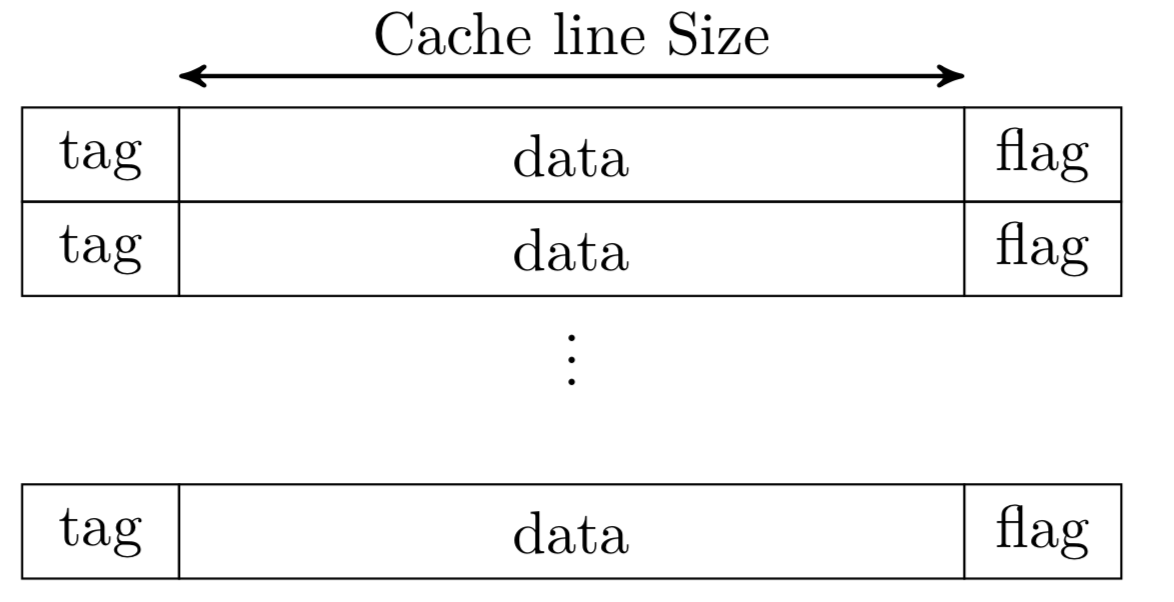
\includegraphics[width=8cm]{images/cacheline_def.png}
    \caption{\label{pic:cacheline} Représentation d'une ligne de cache.}
\end{figure}


%%%%%%%%%%%%%%%%%%%%%%%%%%%%%%%
\subsection{Performances de la hiérarchie mémoire}
%%%%%%%%%%%%%%%%%%%%%%%%%%%%%%%
Mal utilisée, la hiérarchie mémoire n'apporte aucun gain de performance. Son efficacité réside dans la présence des données utilisées dans les niveaux de caches les plus proches de la mémoire. Pour cela, tirer avantage du principe de localité présenté ci-dessous est primordial. D'autres techniques (matérielles et logicielles) permettent d'améliorer l'efficacité de la hiérarchie en réduisant la latence mémoire et en améliorant l'utilisation du bus mémoire. 


\subsubsection{Localité}\label{sec:locality}
Le principe de localité exprime la faculté d'un programme à utiliser des données présente dans les premiers niveaux de cache. Elle peut être de deux types:
\begin{itemize}
    \item \textbf{La localité spatiale} s'appuie sur l'utilisation de données dont les adresses sont consécutives en mémoire (accès encadré en vert sur la \autoref{pic_cpu_locality}). En effet, la taille d'un bloc de données transféré entre la mémoire (une ligne de cache) mesure plusieurs octets et contient plusieurs éléments. Un programme utilisant des données consécutives en mémoire, aura la chance de trouver la donnée suivante déjà chargée dans le cache. 
    \item \textbf{La localité temporelle} exprime la réutilisation d'une donnée dans un futur proche, augmentant la probabilité qu'elle soit toujours dans le cache (accès encadré en bleu sur la \autoref{pic_cpu_locality}). Par exemple, les instructions d'un programme se suivent en mémoire et sont accédées consécutivement. 

\end{itemize}

Le programmeur doit être conscient de ces deux opportunités lorsqu'il écrit son programme. Pour profiter de la localité spatiale, il doit organiser ses données de telle sorte que l'algorithme les parcourt de façon continue. Si la taille de la mémoire le permet, il peut être avantageux de transformer la structure de données, de façon temporaire, pour placer les données utilisées consécutivement en mémoire. Pour profiter de la localité temporelle, le programmeur doit veiller à que le maximum d'opération soit exécuté sur une ligne de cache lorsqu'elle se trouve dans la mémoire cache. Il peut alors être utile de réorganiser une boucle de traitement. Cependant, des applications ne peuvent pas, par nature, profiter des localités temporelle et spatiale comme en cryptographie ou analyse de signaux. Ces applications accèdent à des jeux de données immenses de façon aléatoire ne pouvant pas tenir dans les caches, rendant ces derniers inutiles.


\begin{figure}
    \center
    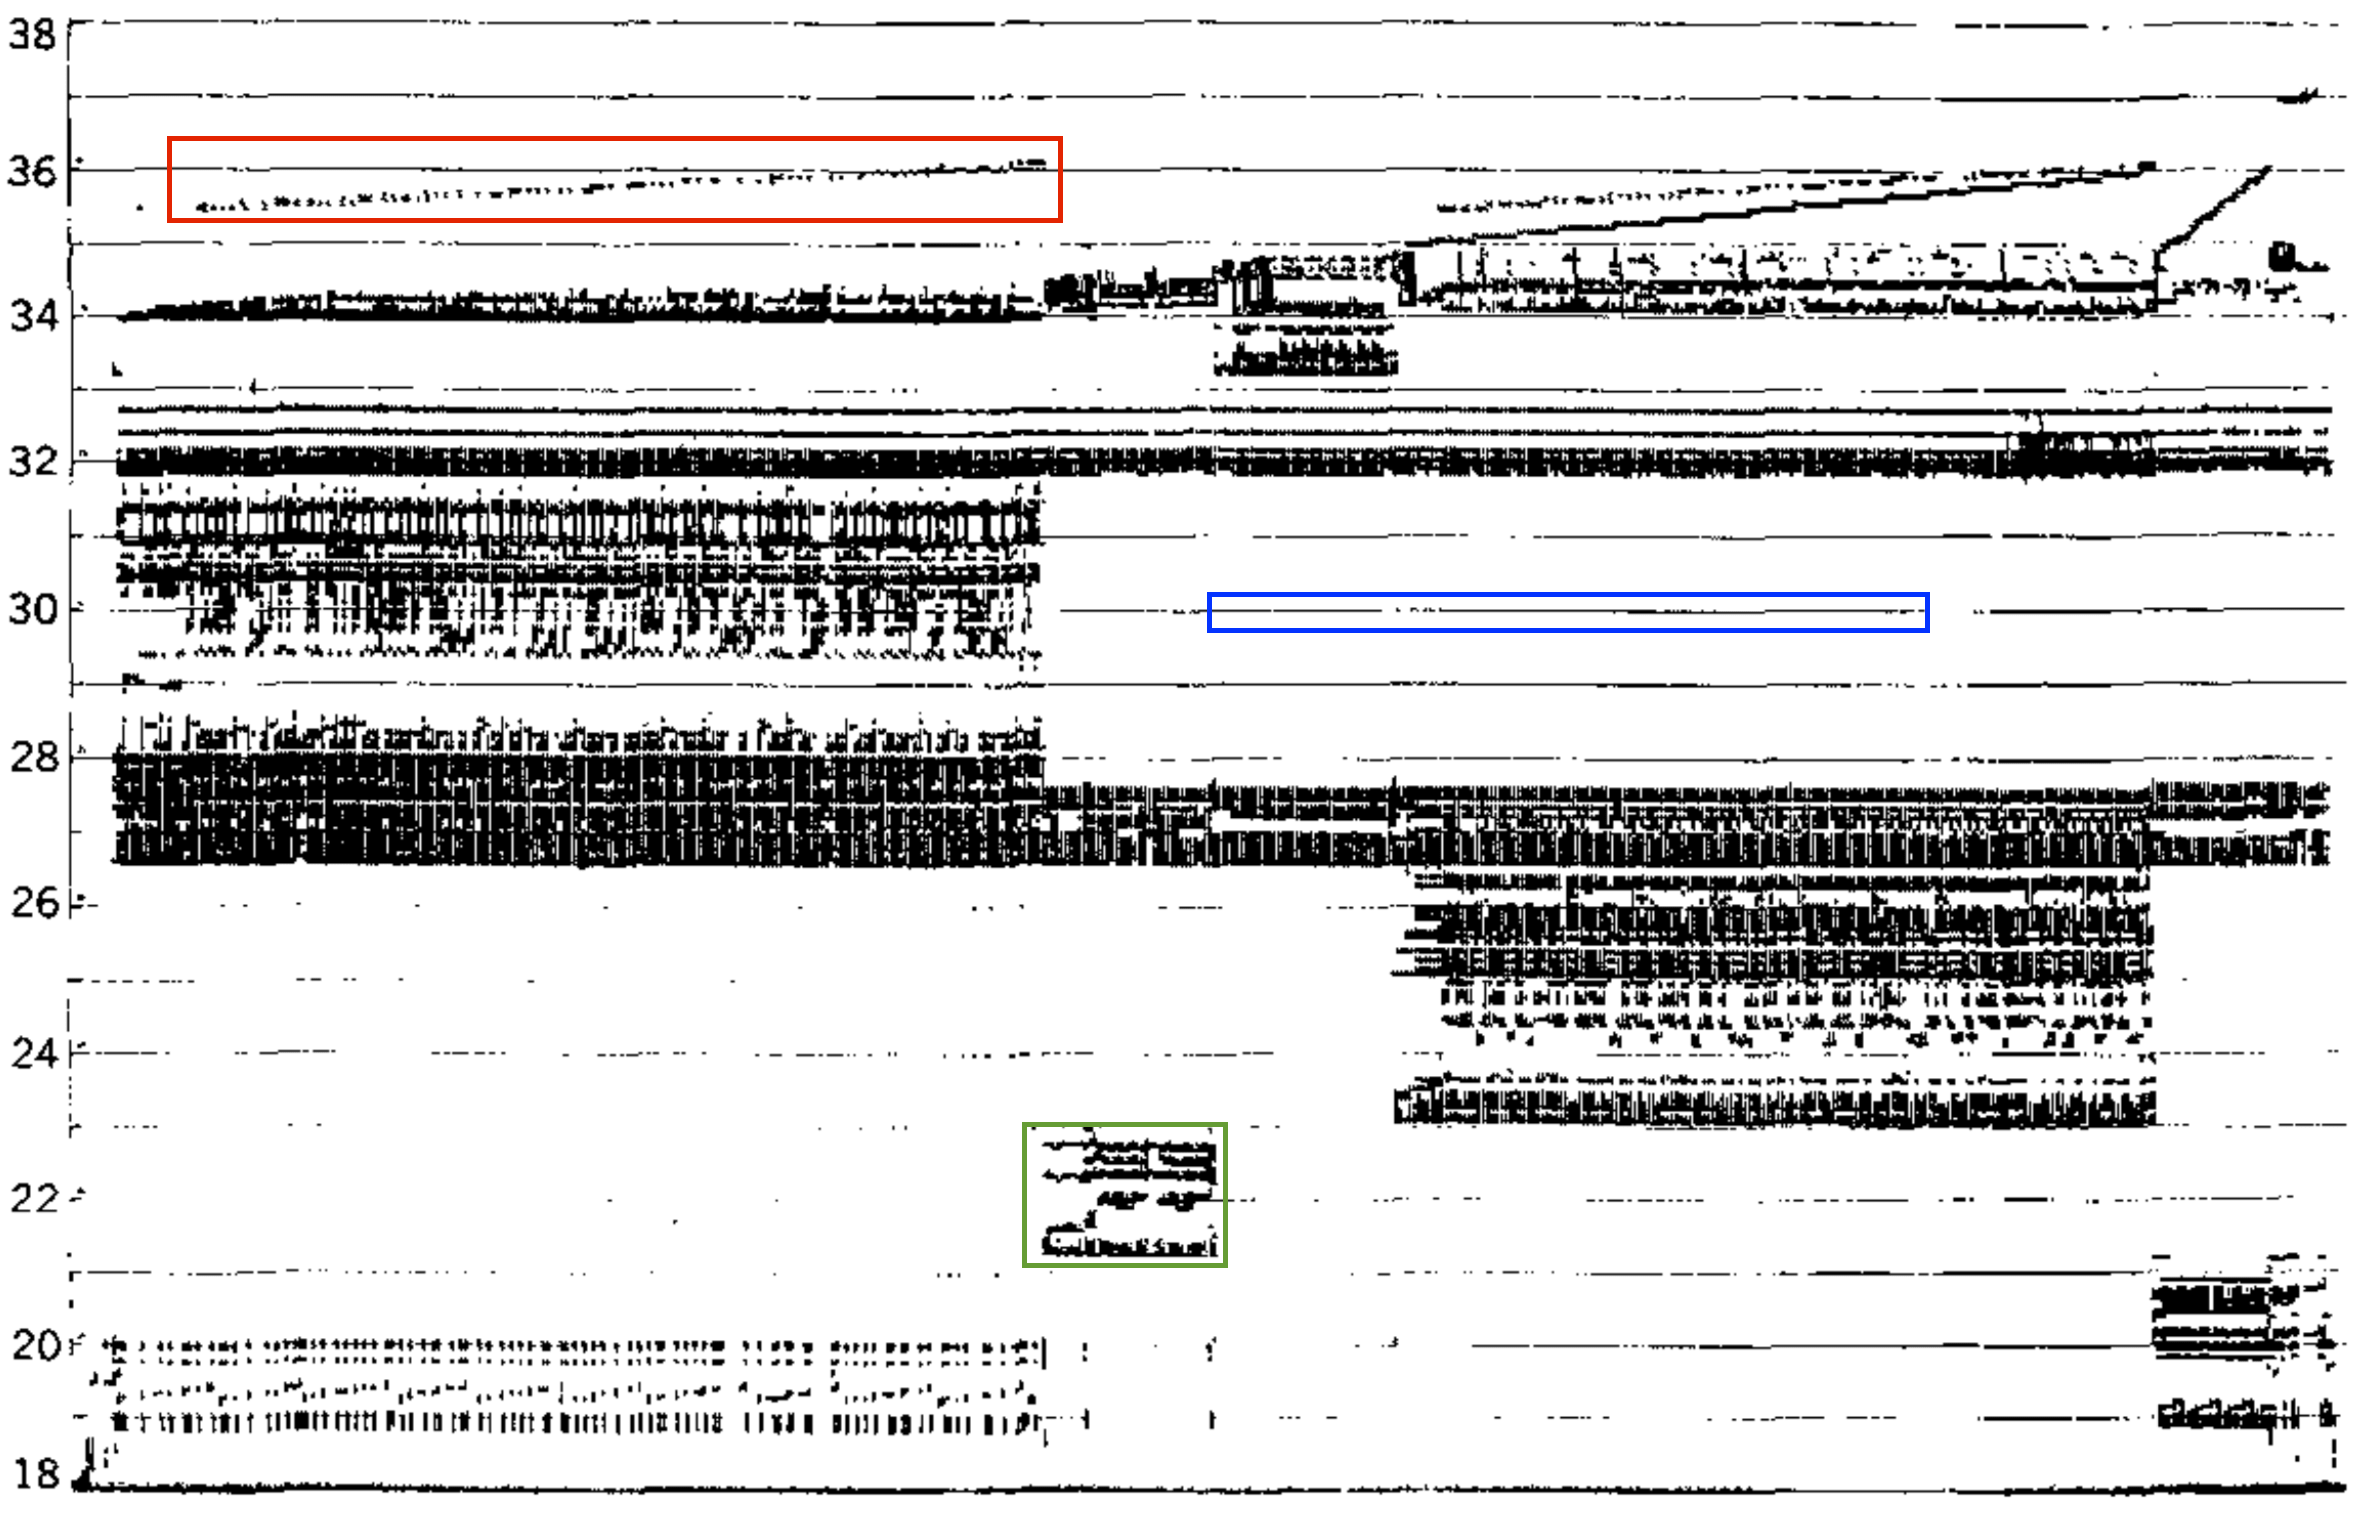
\includegraphics[width=14cm]{images/cpu_locality.png}
    \caption{ Évolution du numéro des pages accédé (axe des ordonnées) en fonction du temps (axe des abscisses) tiré de \cite{Hatfield:1971}. Les accès encadrés en bleu ont une localité temporelle. Les accès encadrés en vert ont une localité spatiale. Les accès encadrés en rouge ne profitent d'aucune localité: 
    \label{pic_cpu_locality}}
\end{figure}




\subsubsection{Saturation du bus mémoire}
%%%%%%%%%%%%%%

Les performances des applications étant principalement limitées par le bus mémoire, il est important que ce dernier soit utilisé à son maximum. On parle alors de \textit{saturation} du bus mémoire. Pour y parvenir, le processeur doit lancer un certain nombre de lecture/écriture dans un petit intervalle de temps. L'application peut, par nature, effectuer suffisamment de transferts mémoires. Sinon des techniques de \textit{prefetching} ou d'injection dans le cache pourront être utilisées. Pour comprendre le lien entre la saturation du bus et la latence mémoire nous utilisons la loi de Little \cite{Little_1961}.

\paragraph{Loi de Little.}\label{sec:loidelittle} Cette loi énoncée en 1961 est utilisée dans la théorie des files d'attente. Elle sert à caractériser le nombre de personnes $N$ dans un système stable (comme une file d'attente), en fonction du temps de traitement $L$ et du débit moyen de client $T$. Le nombre de personnes dans la file peut être calculé par la loi de Little (voir \autoref{eq:little}). Ainsi, pour réduire le temps d'attente d'un client dans une file, il faut soit réduire le nombre de personnes présentes simultanément dans la queue, ou augmenter la cadence de traitement.

\begin{equation} \label{eq:little}
    N = L \times T
\end{equation}

Bien qu'en apparence éloignée du domaine des ordinateurs, cette loi est fondamentale pour comprendre la performance du bus mémoire. Le bus mémoire peut être vu comme une file d'attente dont les clients sont des requêtes mémoires en attente, le temps de traitement est la latence mémoire et le débit représente la bande passante mémoire. La latence et le débit mémoire sont donnés par les caractéristiques de l'architecture. Le but du programmeur est d'utiliser la performance maximale du bus mémoire. Il doit pour cela générer suffisamment de transactions mémoires permettant sa saturation.

Prenons l'exemple d'un bus mémoire ayant une bande passante de 128 GB/s transférant des lignes de cache de 64 bytes et une latence mémoire de 100ns. Son débit est alors de 2 lignes de cache par nanoseconde. Avec la loi de Little, il est possible de calculer le nombre de requêtes mémoires concurrentes nécessaires pour saturer la bande passante mémoire. Dans notre exemple, il est égal à $100 \times 2 = 200$ transactions. 
Si le code, ou l’architecture n’est pas capable de générer, au minimum, 200 requêtes mémoires chaque nanoseconde, le bus mémoire ne pourra jamais être saturé. Un autre impact est que si un processeur est capable de les générer, lui ajouter des coeurs, ne permettra pas d’obtenir de meilleures performances du bus. Pour certains codes limités par la bande passante, il peut être intéressant d’éteindre certains coeurs pour limiter la consommation du processeur sans affecter la performance du code.


\begin{figure}
    \center
    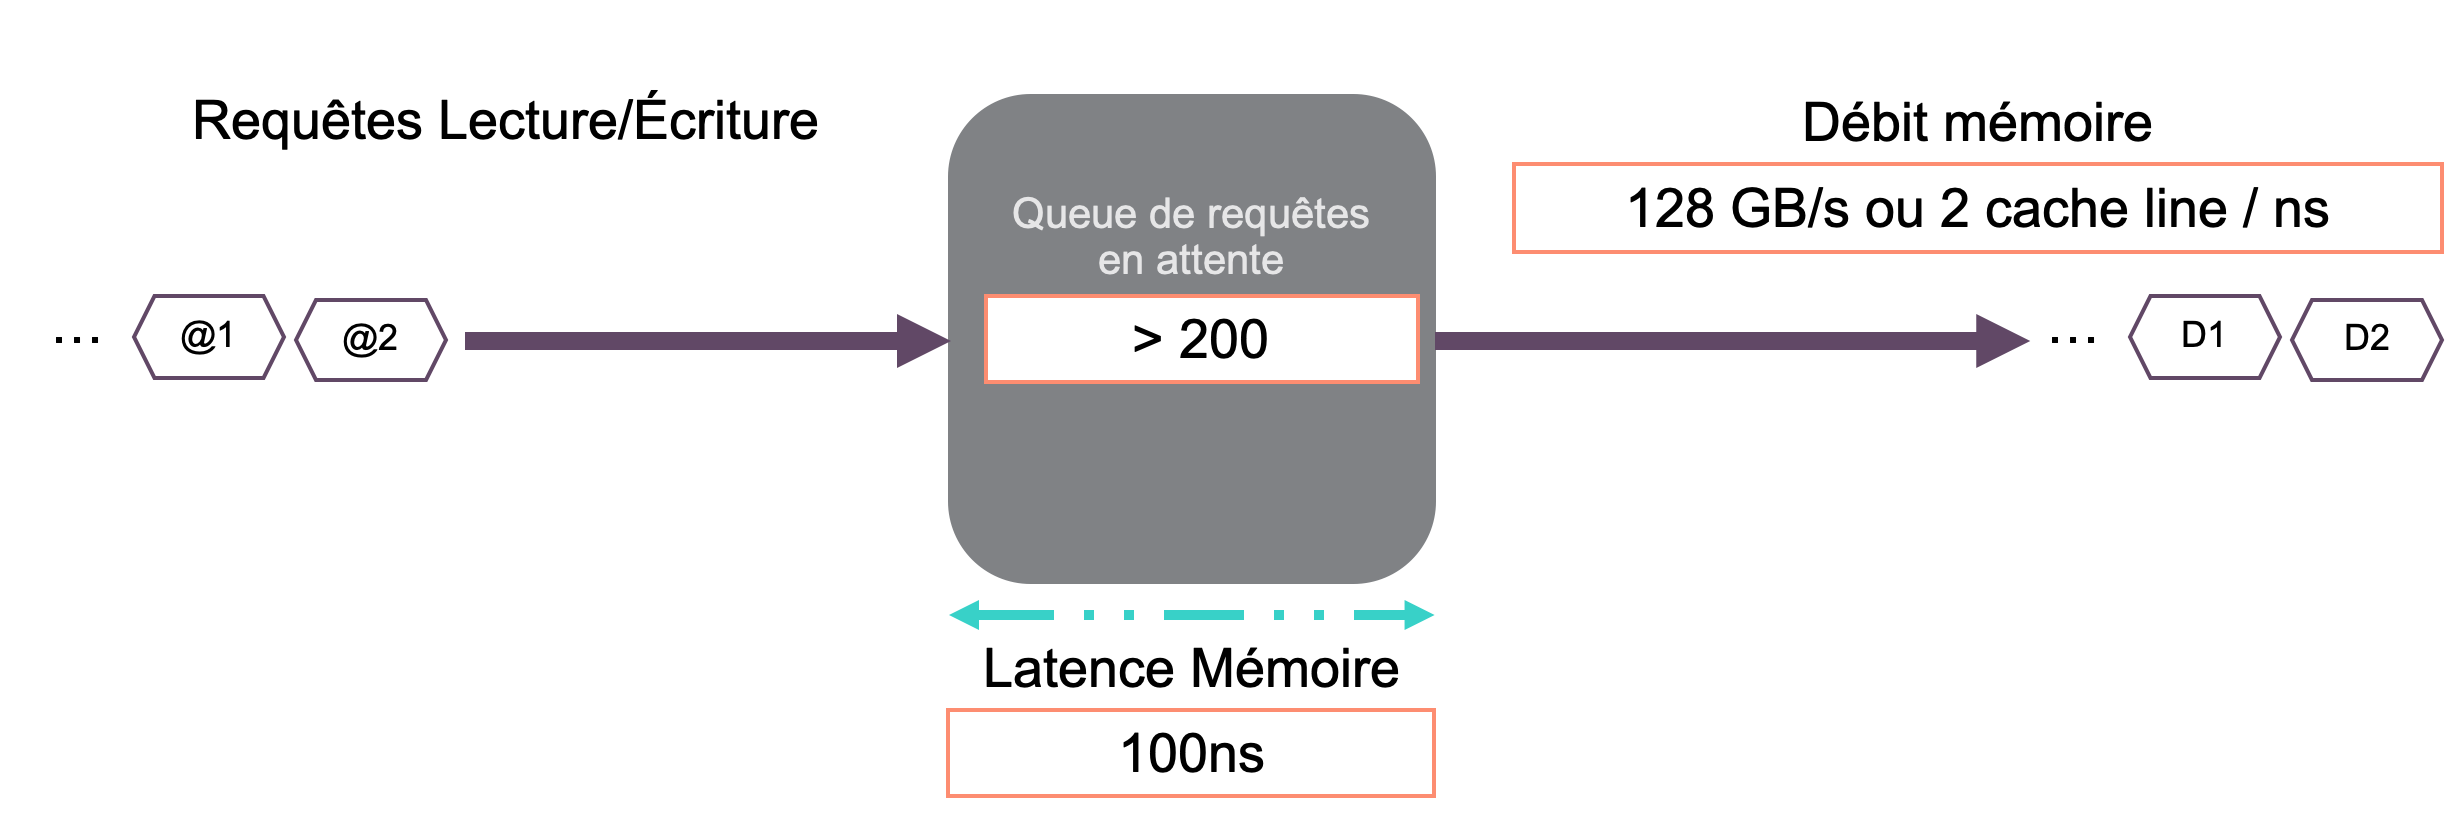
\includegraphics[width=12cm]{images/cpu_littlelaw.png}
    \caption{ La loi de Little permet de calculer le nombre de requêtes mémoires nécessaire pour saturer le bus mémoire. Pour un bus mémoire de 128 GB/s et une latence mémoire de 100ns, il faut qu'il y ait plus de 200 requêtes mémoires en attente pour que le bus soit saturé.
    \label{pic_cpu_littlelaw}}
\end{figure}

Cette loi à un impact direct sur les architectures modernes utilisant des mémoires HMB. Ces mémoires ont des latences d’accès un peu plus faible dû à leur proximité du processeur. Les débits mémoires sont eux aussi bien meilleurs. La loi de Little, implique que le nombre d’accès mémoire à concurrent nécessaires pour saturer ces bus va fortement augmenter. Malheureusement, la microarchitecture actuelle des processeurs n’est pas forcément adaptée à de telles évolutions. Ainsi, nous avons rencontré des architectures incapables de saturer la bande passante mémoire disponible. 

%%%%%%%%%%%%%%%%%%%%%%%%%%%%%%%%%%%%%%%%%%%%%%%%%%%%%%%%%%%%%%%%%%%


\subsection{Caches} \label{sec:cache}
%%%%%%%%%%%%%%%%%%%%%%%%%%%%%%%%%%%%%%%%%%%%%%%%%%%%%%%%%%%%%%%%%%%
%%%%%%%%%%%%%%%%%%%%%%%%%%%%%%%%%%%%%%%%%%%%%%%%%%%%%%%%%%%%%%%%%%%
%intro
C'est en 1965 que les premières mémoires caches sont présentées sous le nom de \textit{slave memory} \cite{wilkes1965slave}. Leur temps d'accès est de 4 à 20 fois plus rapide que celui de la mémoire principale servant alors de mémoire tampon. Cependant, leur taille est très réduite (quelques MiB) comparée à celle de la mémoire principale (plusieurs GiB). Les caches utilisent généralement de la mémoire SRAM.

%performance
Ce niveau de mémoire a été implémenté pour réduire, du point de vue du processeur, l'écart de performance entre ses unités de calculs et celles de la mémoire centrale. Leur apport de performance vient de la capacité des programmes à réutiliser des données déjà présentes dans le cache, évitant un accès à la mémoire centrale beaucoup plus long. Lorsque le processeur doit accéder à une donnée, il commence par la chercher dans le premier niveau de cache, si elle s’y trouve, son temps d'accès est très rapide (événement \textit{cache hit}). Si ce n'est pas le cas (événement \textit{cache miss}), il réalise alors une copie de la zone mémoire la contenant dans le cache. La zone mémoire copiée est appelé \textit{ligne de cache}. Si par la suite, cette donnée ou une donnée appartement à la même ligne de cache devait être à nouveau accédée, leur temps d'accès serait alors drastiquement réduit. Ce mécanisme est transparent pour l'utilisateur, bien que pour des questions de performances il doive être conscient de son existence (voir \autoref{sec:locality}). 

%taille vs performance
La taille de chaque niveau de cache varie pour les raisons expliquées en introduction de cette partie. À cela vient s'ajouter la notion de performance qui est liée à leur taille. Un cache de grande capacité aura plus de chance de contenir la donnée dont le processeur a besoin, améliorant ainsi la performance moyenne du programme. Un cache est une mémoire associative. Pour accéder à son contenu, il faut utiliser une clef associative. La clef est constituée de l'adresse en mémoire centrale de l'instruction ou de la donnée.

Pour allier les avantages et contourner les inconvénients, les processeurs utilisent non pas un, mais plusieurs niveaux de caches de tailles différentes.
Le premier niveau de cache est généralement séparé en deux zones mémoire: l'une contenant les instructions et l'autre les données. C'est le seul niveau de la hiérarchie qui stocke différemment les données et les instructions. Sur les processeurs récents, le premier et le deuxième niveau de cache est privé à chaque coeur. Un troisième et parfois un quatrième niveau de cache est partagé entre les différents coeurs du processeur. La \autoref{pic:cache_hierarchy} représente une telle architecture pour un processeur à 4 coeurs. Le partage d'un ou plusieurs niveaux de caches entre différents coeurs à certains bénéfices en programmation parallèle. La communication entre les coeurs est plus rapide, ainsi que la migration d'un thread entre deux coeurs partageant un même niveau de cache. Cependant, cela introduit de la complexité pour la cohérence des caches (voir \autoref{sec:cache_coherence}).


\begin{figure}
    \center
    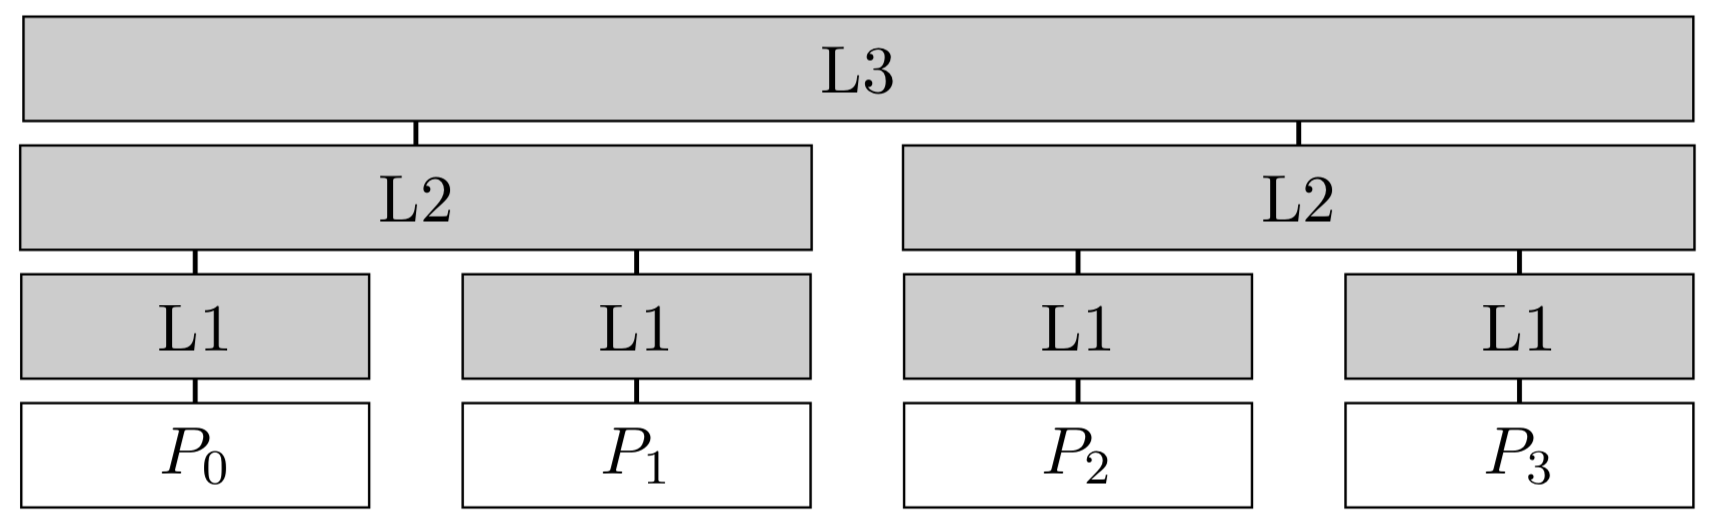
\includegraphics[width=8cm]{images/cache_hierarchy.png}
    \caption{\label{pic:cache_hierarchy} Organisation d'une hiérarchie de caches à trois niveau sur un processeur à 4 coeurs (source \cite{putigny2014benchmark}).}
\end{figure}




\subsubsection{Propriété d'inclusion}
%%%%%%%%%%%%%%%%%%%%%%%%%%%%%%%%%%%%%%%%%%%%%%%%%%%%%%%%%%%%%%%%%%%
Lorsqu'une donnée est chargée depuis la mémoire, le processeur doit la stocker dans le cache qui varie en fonction de la propriété d'inclusion du processeur pouvant être inclusive ou exclusive ou non inclusive.

Un cache est dit inclusif, si lorsqu'une donnée se trouve à un niveau de la hiérarchie, tous les caches des niveaux supérieurs contiennent eux aussi une copie de la donnée (voir \autoref{pic:InclusivePolicy}). Cette politique d'inclusion a un désavantage lorsqu'elle est utilisée sur des systèmes multi-coeurs. En effet, lorsqu'une donnée doit être retirée d'un niveau de cache, le processeur doit aussi l'enlever des niveaux de caches inférieurs.  Un cache non-inclusif permet qu'une ligne du cache de niveau 1 ne soit pas forcément dans le cache de niveau 2. Cela permet d'augmenter la capacité de la hiérarchie de cache. Les processeurs récents implémentent les deux politiques d'inclusion. Le processeur Intel Sandy Bridge a un cache L3 inclusif tandis que les caches L1 et L2 sont non-inclusif. Pour une politique d'exclusion, une donnée qui se trouve à un niveau du cache ne peut pas se trouver dans un autre niveau de cache au même moment (voir \autoref{pic:ExclusivePolicy}). L'avantage des caches exclusif est leur capacité de stocker plus de données, car une ligne de cache ne se trouve jamais à deux endroits à la fois de la hiérarchie de cache. Cependant, lors d'un \textit{hit} dans le cache L2, le processeur doit échanger la ligne entre les deux niveaux de cache L1 et L2, plus long qu'une simple copie.




\begin{figure}
    \centering
    \begin{subfigure}[b]{0.45\linewidth}
        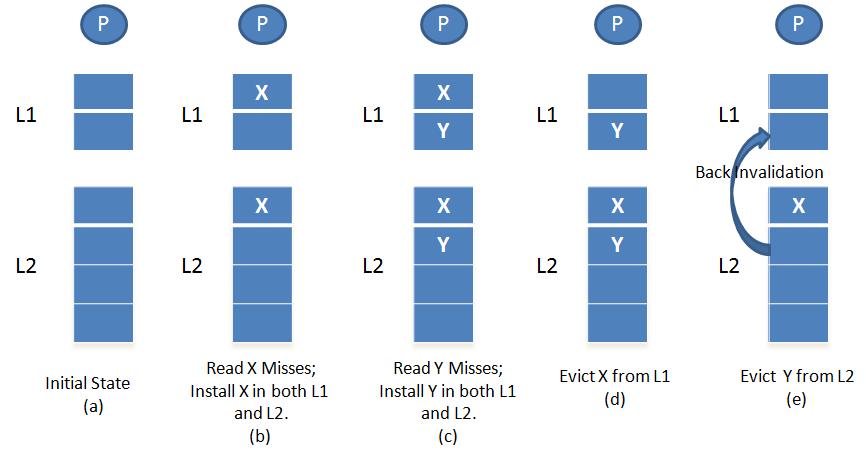
\includegraphics[width=\linewidth]{images/InclusivePolicy.png}
        \caption{Inclusive}
        \label{pic:InclusivePolicy}
    \end{subfigure}
    ~ %add desired spacing between images, e. g. ~, \quad, \qquad, \hfill etc. 
      %(or a blank line to force the subfigure onto a new line)
    \begin{subfigure}[b]{0.45\linewidth}
        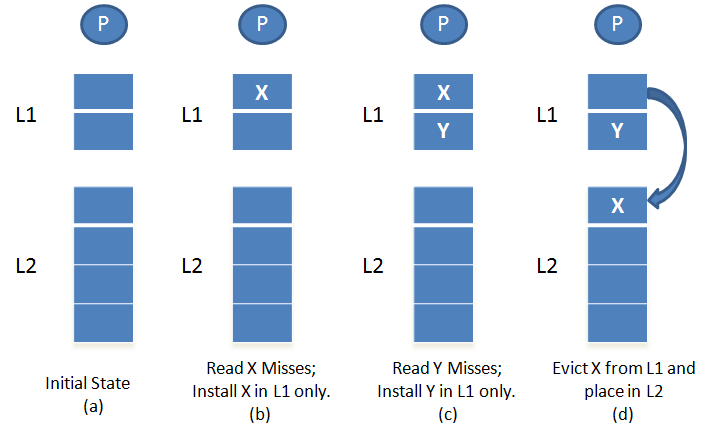
\includegraphics[width=0.85\linewidth]{images/ExclusivePolicy.png}
        \caption{Exclusive}
        \label{pic:ExclusivePolicy}
    \end{subfigure}
    \caption{Exemple de deux propriétés d'inclusion de la hiérarchie de cache (source \cite{wikipedia_2019}). }\label{fig:cacheinclusionpolicy}
\end{figure}




\subsubsection{Politique de placement: associativité}
%%%%%%%%%%%%%%%%%%%%%%%%%%%%%%%%%%%%%%%%%%%%%%%%%%%%%%%%%%%%%%%%%%%
La performance d'un cache ne vient pas seulement de la technologie utilisée pour sa construction. En effet, lorsqu'une donnée est accédée, le cache doit vérifier si la donnée est présente ou non dans le niveau de cache demandé. Il faut que l'algorithme de comparaison permettant de la trouver soit le plus rapide possible. Pour cela, les architectes utilisent généralement une fonction de \textit{hash} permettant d'attribuer un emplacement dans le cache en fonction de l'adresse mémoire de la \textit{cache line}. Si la \textit{cache line} ne se trouve pas à l'emplacement calculé, c'est quelle n'est pas présente dans ce niveau de cache.


\begin{figure}
    \centering
    \begin{subfigure}[b]{0.45\linewidth}
        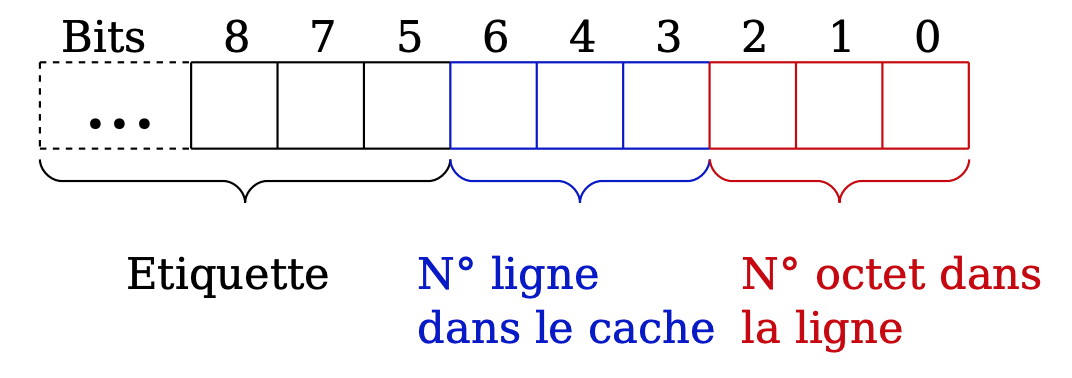
\includegraphics[width=\linewidth]{images/cache_calcul.png}
        \caption{Calcul de l'emplacement (index de la ligne et décalage) pour un mappage direct}
        \label{pic:cache_calcul}
    \end{subfigure}
    ~ %add desired spacing between images, e. g. ~, \quad, \qquad, \hfill etc. 
      %(or a blank line to force the subfigure onto a new line)
    \begin{subfigure}[b]{0.45\linewidth}
        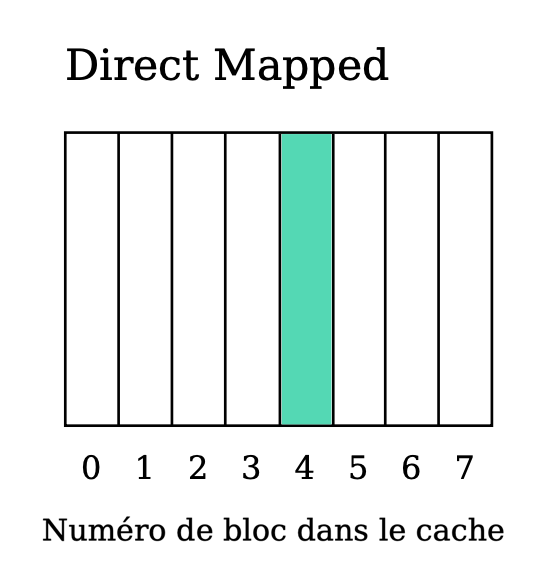
\includegraphics[width=\linewidth]{images/cache_direct.png}
        \caption{Emplacement de la ligne calculée dans le cache ou sera stockée la \textit{cache line}.}
        \label{pic:cache_direct}
    \end{subfigure}
    \caption{Exemple du calcul de l'emplacement de la ligne de cache lors d'un mappage direct à partir de l'adresse de la \textit{cache line} à stocker (source \cite{Meunier2017}). }\label{fig:cacheinclusionpolicy}
\end{figure}





Les trois politiques de placement les plus utilisées sont: le mappage  \textit{direct }, le mappage \textit{fully associative} et le mappage \textit{set assiociative} (voir \autoref{pic:cache_associativite}).


\begin{figure}
    \center
    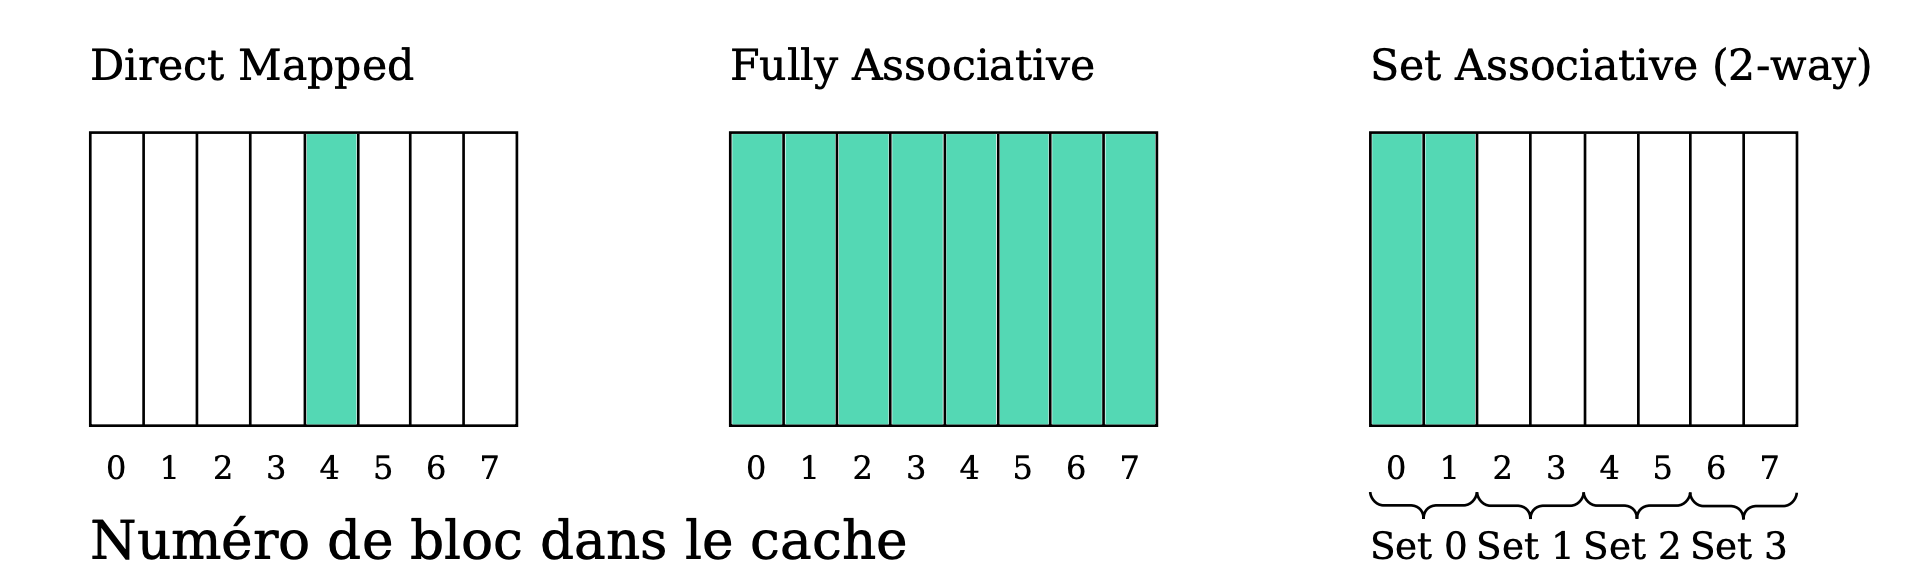
\includegraphics[width=12cm]{images/cache_associativite.png}
    \caption{\label{pic:cache_associativite} En fonction de la politique de remplacement utilisée, une \textit{cache line} sera associée à une ligne du cache différente (source \cite{Meunier2017})}
\end{figure}

\paragraph{Cache à correspondance directe (\textit{direct-mapped cache})} utilise une fonction simple pour déterminer l'emplacement (index et offset) du cache à utiliser. Une partie des bits le l'adresse de la \textit{cache line} est utilisée pour déterminer la ligne à utiliser (\textit{index}) par exemple à l'aide d'une opération modulo. L'autre partie est utilisée pour déterminer le décalage dans cette ligne (\textit{offset}). Cette méthode est très rapide, mais peut avoir des performances catastrophiques. Un algorithme faisant des sauts en mémoire d'une certaine taille pourrait n'utiliser qu'une seule ligne du cache, le rendant totalement inefficace. Comparé aux caches associatifs, le mappage direct est plus simple à implémenter, car un seul comparateur est nécessaire pour déterminer la ligne de cache à utiliser (voir \autoref{fig:cache_schema}).

\paragraph{Cache pleinement associatif (\textit{fully associative cache})} remédie à ce problème en permettant à une \textit{cache line} d'être stockée à n'importe quel emplacement dans le cache. Ainsi, la totalité du cache peut être utilisée. Cependant, cette technique a le désavantage d'être très lente. En effet, une \textit{cache line} pouvant se trouver à n'importe quelle ligne du cache, il faut toutes les comparer pour vérifier sa présence ou non. Pour faire cette comparaison en parallèle, il faudrait implémenter autant de comparateurs que de ligne dans le cache, complexifiant grandement le cache.

\paragraph{Cache N-associatif (\textit{N-way set associative cache})} permet de réduire le nombre de comparateurs nécessaires en regroupant les lignes du caches potentiellement adressable pour une \textit{cache line} en groupe (\textit{set}). L'exemple de la \autoref{pic:cache_associativite} utilise un cache à 4 set, appelé \textit{4-way associative}. Il ne faut plus que 4 comparateurs pour déterminer si une ligne appartient à un des \textit{set}. Les mappages par association sont plus lents que le mappage direct, car il faut trouver où se trouve la \textit{cache line} (si présente) dans un sous ensemble de ligne de cache plus ou moins grand. Pour accélérer la recherche de la présence ou non d'une ligne de cache, le traitement peut être réalisé en parallèle dans les différents \textit{sets} par l'utilisation de plusieurs comparateurs (4 dans la \autoref{pic:cache_circuit-set-associative}). 

La propriété principale d'un cache est sa capacité à conserver les données pour de futurs accès. Un cache de 8 MB à 2 sets associatifs peut sauver jusqu'à 44\% des \textit{miss} comparé à un cache à correspondance direct \cite{Drepper2007}. Sur les architectures récentes Intel Skylake, les caches utilisent entre 8 et 16 associativités, pouvant varier entre les différents niveaux. 



\begin{figure}
    \begin{subfigure}[t]{\linewidth}\centering
        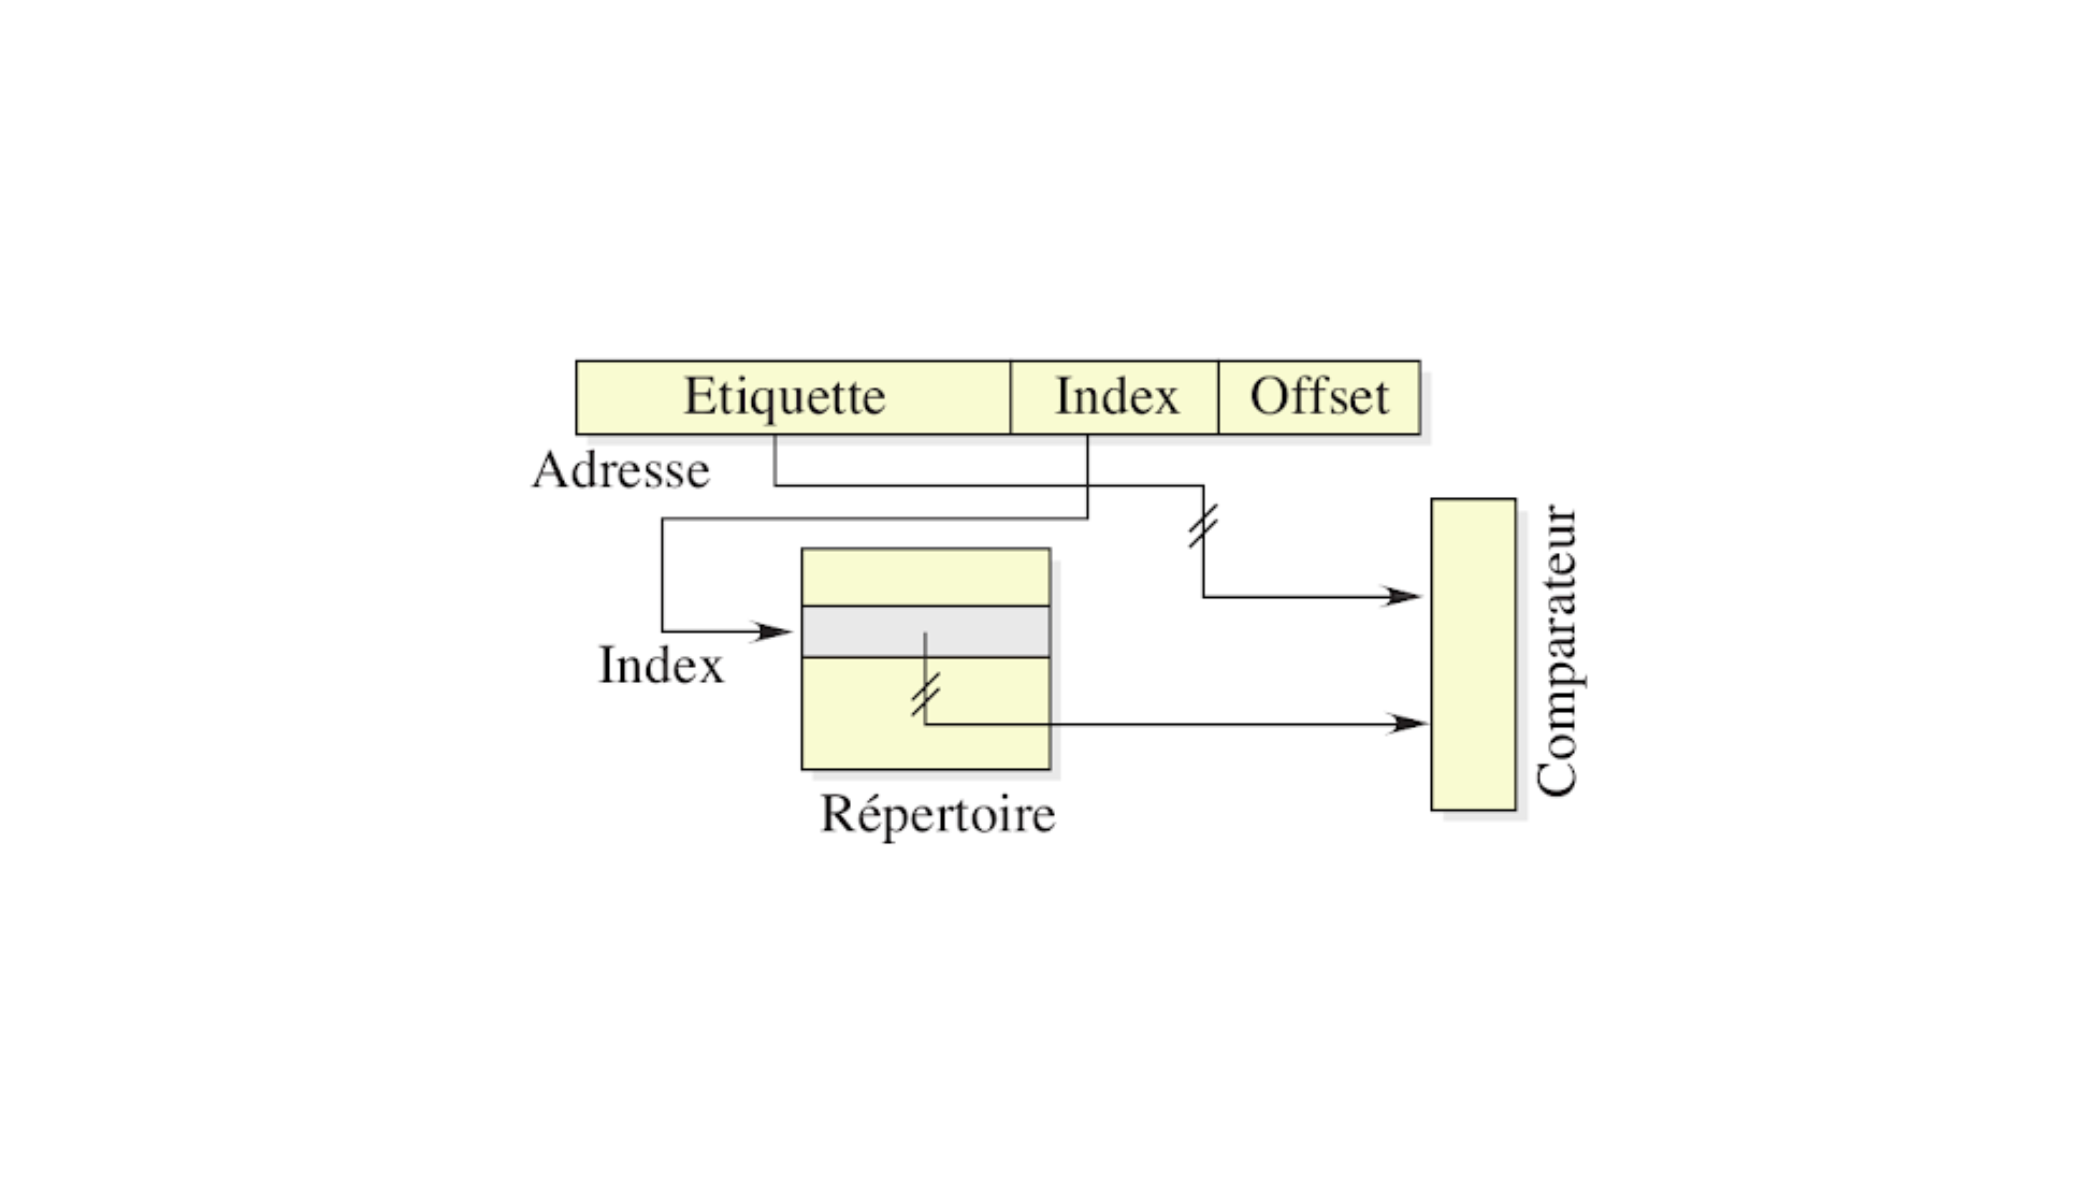
\includegraphics[width=0.7\linewidth, trim = 0cm 10cm 0cm 2cm]{images/cache_circuit-direct.png}
        \caption{Le cache pleinement associatif nécessite d'avoir un comparateur pour chacune des lignes du cache}
        \label{pic:cache_circuit-direct}
        \vspace{1cm}
    \end{subfigure}
    
    \begin{subfigure}[t]{\linewidth}\centering
        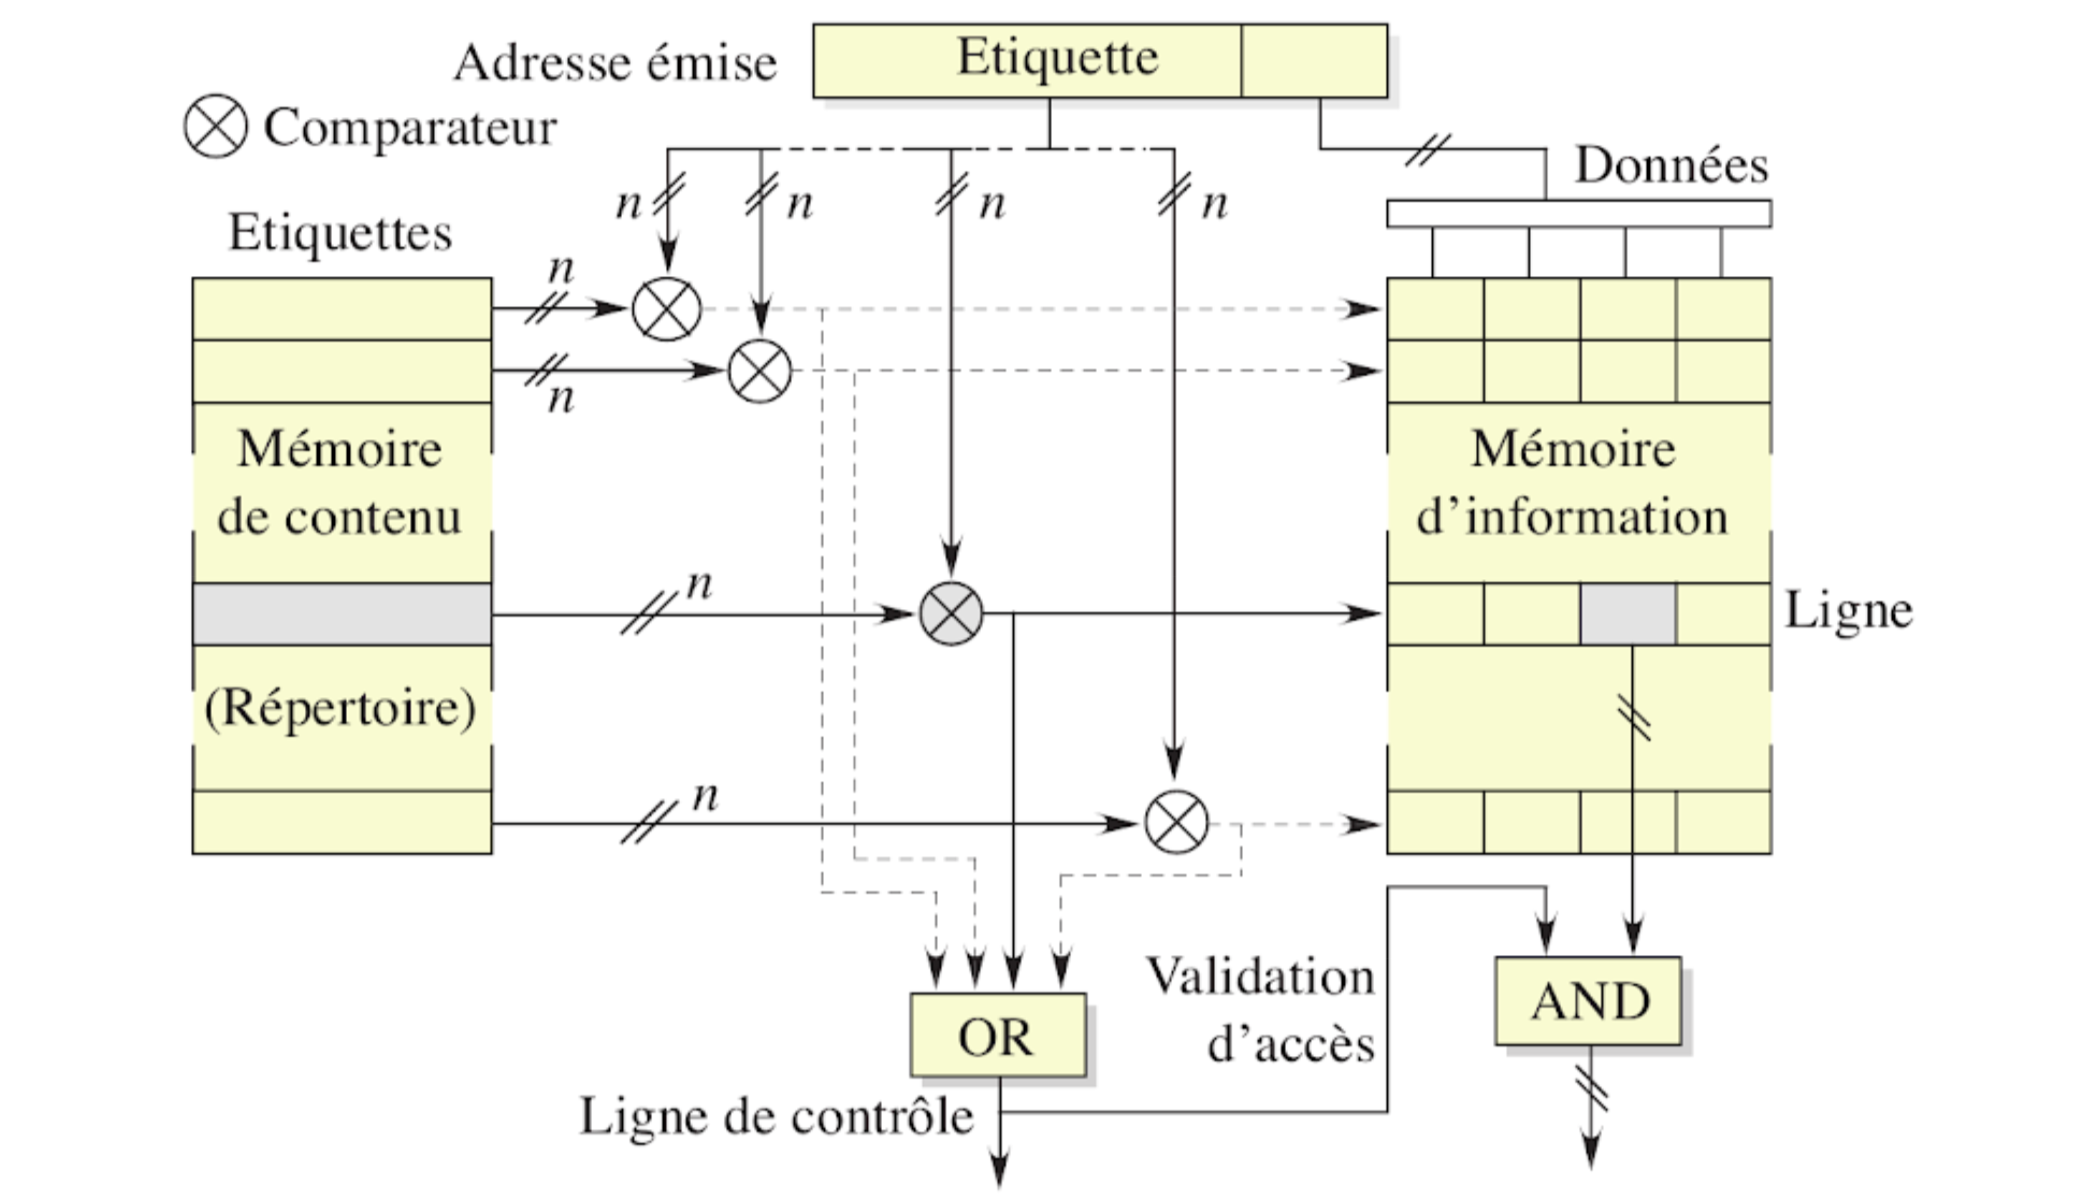
\includegraphics[width=0.7\linewidth]{images/cache_circuit-fully-associative.png}
        \caption{Le cache pleinement associatif nécessite d'avoir un comparateur pour chacune des lignes du cache}
        \label{pic:cache_circuit-fully-associative}
        \vspace{.5cm}
    \end{subfigure}
    
    \begin{subfigure}[t]{\linewidth}\centering
        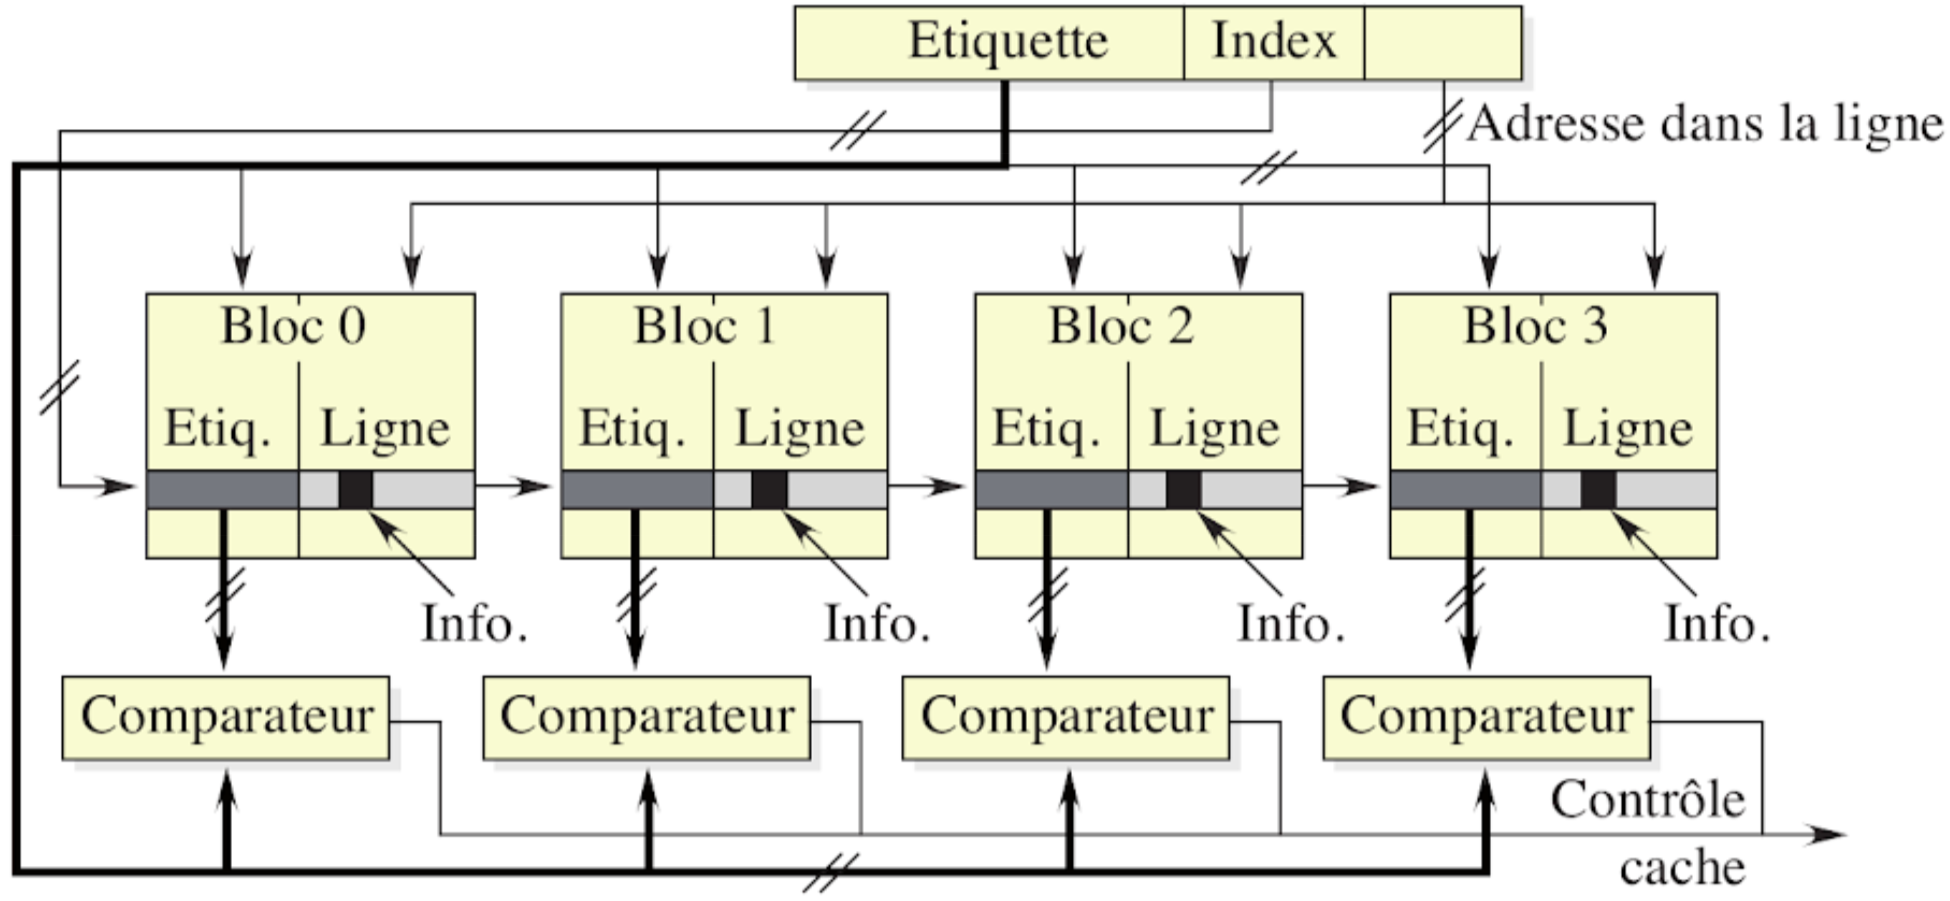
\includegraphics[width=0.7\linewidth]{images/cache_circuit-set-associative.png}
        \caption{Le cache N-associatif associe les deux architectures des caches direct et pleinement associatif. Ce sont plusieurs caches directs montés en parallèles.}
        \label{pic:cache_circuit-set-associative}
    \end{subfigure}
    
    \caption{Schéma des trois modèles de cache utilisés (tirés de l'ouvrage \cite{Blanchet2013}).}\label{fig:cache_schema}
\end{figure}




\subsubsection{Politique de remplacement}
%%%%%%%%%%%%%%%%%%%%%%%%%%%%%%%%%%%%%%%%%%%%%%%%%%%%%%%%%%%%%%%%%%%
Que ce soit pour le mappage \textit{fully associative} ou \textit{set associative}, une \textit{cache line} peut être stockée dans plusieurs lignes du cache. Pour déterminer laquelle choisir pour y placer la \textit{cache line}, différentes stratégies peuvent être utilisées, appelées \textit{politique de remplacement}. L'objectif de ces politiques est de maximiser l'utilisation du cache en prévoyant et en anticipant les futures lignes à être accéder pour ne pas les supprimer du cache. Il existe de nombreuses politiques de remplacement, chacune ayant ses avantages et ses inconvénients \cite{wikipedia2_2019}: FIFO, LIFO, LRU, TLRU, MRU, PLRU, RR, SLRU, LFU, LFRU, LFUDA, LIRS, ARC, CAR, MQ. La politique choisie à un réel impacte sur les performances de l'application. Pour la choisir, il faut trouver un compromis entre la performance et la complexité apportée par sa mise en place. Dans le cas du mappage \textit{direct}, la ligne de cache présente à l'emplacement calculé est forcément remplacée et ne nécessite pas d'avoir une politique de remplacement. Il existe deux familles de politiques de remplacement. La première famille regroupe les politiques de remplacements qui tiennent compte de l'utilisation des \textit{cache line} (LRU, FIFO). Ce sont généralement les politiques les plus efficaces. La deuxième famille est celle des politiques aléatoires (\textit{random}, \textit{round robin}) qui ne tiennent pas compte de l'utilisation des données et choisissent une ligne aléatoirement à remplacer. Ces politiques sont performantes en termes de rapidité d'exécution, car le choix ne se fait que sur une fonction aléatoire. Cependant, \cite{Al-Zoubi:2004:PEC:986537.986601} montrent que ces techniques utilisent 22\% moins bien le cache, impactant les performances des applications.

\paragraph{Least Recently Used} ou LRU remplace la ligne de cache la moins récemment utilisée. Les numéros des lignes utilisées sont stockés dans une pile suivant la date de leur dernière utilisation. La pile est mise à jour lorsqu'une nouvelle donnée est stockée dans le cache en empilant son adresse au sommet de la pile. De même, lors d'un \textit{hit}, la ligne de cache référencé est stockée elle aussi en sommet de pile. Cette méthode à un inconvénient pour certains types d'accès, notamment les parcours de tableau. Imaginons un cache pouvant contenir 4 lignes. Le double parcours d'un tableau mesurant 5 lignes de caches a,b,c,d,e aura les accès mémoire suivants: a,b,c,d,e a,b,c,d,e. Le deuxième accès au tableau ne profitera pas du cache, car chaque ligne de cache est remplacée au fur et mesure du parcours du tableau. Des améliorations ont été apportées pour corriger ce problème, comme l'introduction d'un répertoire image \cite{Stone:1987:HCA:31845} qui garde une trace des groupes de lignes de cache utilisées ensemble pour prévoir les accès similaires et anticiper leur accès.







\subsubsection{Stratégie de cache: lecture et écriture}
%%%%%%%%%%%%%%%%%%%%%%%%%%%%%%%%%%%%%%%%%%%%%%%%%%%%%%%%%%%%%%%%%%%
Le cache est une zone mémoire qui évolue en fonction des accès mémoires. Son fonctionnement lors d'un accès (en lecture ou écriture) peut varier en fonction de la présence (\textit{hit}) ou non (\textit{miss}) de la donnée et de la stratégie de cache implémentée.

\paragraph{Lecture:}  lorsque le processeur accède à une donnée, il vérifie qu'elle n'est pas présente dans ses différents niveaux de cache. Si la donnée est présente, son accès est très rapide. Si ce n'est pas le cas, il réalise alors une copie de la zone mémoire la contenant dans le cache (la taille de la zone est une ligne de cache).

\paragraph{Écriture:} le comportement du cache lors d'une écriture dépend de la présence ou non de la \textit{ligne de cache} et la politique employée.

Si la ligne de cache n'est pas présente (\textit{miss}) dans le cache, deux solutions sont possibles. La première est de charger la ligne depuis la mémoire et d'y apporter les modifications (politique \textit{Write-Allocate}). La deuxième solution est d'écrire la ligne de cache sans la charger (politique \textit{No-Write-Allocate}). La ligne de cache ne sera chargée que lors d'un miss lors d'une lecture, sauf si la totalité de la ligne a été écrite, les données originales n'ayant plus de valeur utile. Cette option peut être intéressante si un algorithme ne fait qu'écrire dans une structure de donnée sans ne jamais la lire.

Si la ligne de cache est présente (\textit{hit}) dans le cache, deux solutions sont possibles. La première est de mettre à jour la \textit{cache line} dans le cache et en mémoire pour que le changement soit répercuté sur l'ensemble de la hiérarchie mémoire (politique \textit{Write-Through}). Cette politique peut être pénalisante si le processeur effectue consécutivement la mise à jour d'une donnée (par exemple un compteur, ou un index de boucle).  La seconde solution est de différer l'écriture à plus tard (politique \textit{Write-Back}). L'écriture est effectuée seulement dans le cache et ne sera effective en mémoire seulement lorsque la ligne de cache modifiée sera évincée du cache. La ligne de cache modifiée est alors indiquée grâce à un bit indicatif (\textit{dirty bit}). Comparée à la première méthode, celle-ci utilise moins de bande passante, car les mises à jour en mémoire sont moins fréquentes. Cependant, si plusieurs coeurs utilisent la même donnée, sa valeur pourrait alors être différente entre leurs caches respectifs (donnée périmée). Il faut alors implémenter un protocole de cohérence de cache entre les différents caches et la mémoire.

Les politiques utilisées lors d'un \textit{miss} ou d'un \textit{hit} peuvent être associés. Les combinaisons les plus utilisées sont \textit{Write-Through} + \textit{No-Write-Allocate} et \textit{Write-Back} + \textit{Write-Allocate}.






\subsubsection{Cohérence de cache} \label{sec:cache_coherence}
%%%%%%%%%%%%%%%%%%%%%%%%%%%%%%%%%%%%%%%%%%%%%%%%%%%%%%%%%%%%%%%%%%%

La stratégie employée lors de la modification d'une donnée introduit un challenge majeur des architectures multi-coeurs qui est de garantir la cohérence des données entre les différentes zones mémoires. Lors d'un accès mémoire, on souhaite accéder à la valeur la plus récente, qui aura pu être modifiée par un autre coeur, ou processeur. La gestion de la cohérence d'un processeur à un seul coeur est plus simple, bien qu'elle doive tout de même être implémentée. Les opérations d'entrée-sortie peuvent affecter des données en mémoire qui se trouve aussi dans les caches.

Le protocole de cohérence de cache est responsable de vérifier qu'une même ligne de cache présente à plusieurs emplacements de la mémoire est identique. Il doit pour cela garantir trois points. Le premier est de partager le changement d'une valeur à tous les coeurs d'un processeur pour que l'ordre des opérations affecté à une valeur soit vu dans le même ordre par tous les coeurs/processeurs. Le deuxième point est d'assurer que le résultat ne dépende que de l'ordre des instructions du programme assembleur et non de l'ordre de leur exécution par les différents coeurs. Enfin, le protocole doit assurer à un coeur qui lit une donnée que sa valeur est bien la dernière qui a été écrite (par un autre coeur ou autre processeur). La notion d'ancienneté peut être définie de plusieurs façons et le protocole doit la définir précisément pour assurer la validité des résultats \cite{Blanchet2013}. En effet, l'ordre peut faire référence à l'ordre des instructions dans le programme source. L'ordre peut aussi faire référence à celui de la fin des exécutions des résultats (avant que la donnée soit effectivement écrite). Enfin, ce peut être l'ordre des écritures mémoires. Comme la durée de propagation des écritures n'est pas constante dans le système, des erreurs peuvent apparaître si un protocole venait à utiliser ce dernier.

Comme le résume \cite{Blanchet2013}, les deux propriétés principales d'un protocole de cohérence sont sa simplicité de mise en oeuvre et sa performance. Pour assurer la cohérence, deux familles de protocoles existent, suivant si la gestion de cohérence est répartie sur les différents caches (\textit{locale}), ou si elle est centralisée (\textit{globale}). 


\paragraph{Protocoles locaux - cohérence répartie}

Les protocoles \textit{locaux} utilisent des outils de scrutation (\textit{snooping}) et de signalisation (\textit{broadcasting}). Implémentés directement dans les caches, ils ne nécessitent pas la modification ni de la mémoire ni du processeur. Lorsqu'une \textit{cache line} est modifiée dans un cache, il obtient la copie exclusive de celle-ci en invalidant ses copies dans d'autres caches (\textit{Write-Invalidate}). Une seconde option vise à simplement signaler la modification de cette ligne aux autres caches pour qu'ils mettent à jour leur structure de donnée (\textit{Write-Update}).  Différents protocoles de cohérence ont été implémentés et ont évolué. Les plus connues sont les protocoles MESI (ou \textit{Illinois}) \cite{papamarcos1984low} et MOESI. Mais il en existe beaucoup d'autres: MSI, MOSI, MERSI, MESIF. MESI et MOESI sont notamment très utilisés dans les processeurs multi-coeurs car il implémente des stratégies à écriture différée, minimisant le trafic mémoire.
\\
Nous présentons le protocole \textit{MOESI} à titre d'exemple. \textit{MOESI}  permet à une ligne de cache d'avoir cinq états différents. Le passage entre les différents états est résumé dans la \autoref{pic:moesi}. Chaque coeur surveille toutes les commandes effectuées sur le bus pour mettre à jour l'état de ses lignes ou les communiquer quand il en est propriétaire.

L'état $M$ (\textit{modified)} indique que la ligne est valide et qu'elle a été modifiée dans ce niveau de cache et qu'elle est seulement présente dans ce cache. La valeur en mémoire n'est pas cohérente, la ligne doit alors être copiée en mémoire lors de son remplacement. 

L'état $O$ (\textit{owned} ou \textit{shared-modified}) indique que cette ligne est valide est qu'elle est présente dans au moins un autre niveau de cache. Le cache actuel est \textit{propriétaire} de cette ligne, il doit informer les autres caches lors de sa modification. La ligne modifiée peut ensuite être communiquée à un autre niveau de cache, sans avoir à passer par la mémoire. Cet état est la principale amélioration apportée par le protocole \textit{MOESI} au protocole \textit{MESI}.

L'état $E$ (\textit{exclusive}) indique que la ligne est valide uniquement dans ce niveau de cache. Cela évite l'émission d'invalidation aux autres caches qui ne détiennent pas cette ligne. De plus, sur un autre cache y accède, la ligne de cache peut directement être transférée depuis le cache sans accès mémoire. La ligne dans le premier cache passera alors de l'état $E$ à $O$. Dans le deuxième cache la ligne sera en état $S$.

L'état $S$ (\textit{shared}) indique que la ligne est valide dans le cache courant et dans au moins un autre cache. Le cache actuel n'est pas propriétaire de la ligne (état $O$). La cohérence avec la mémoire n'est pas assumée. 

L'état $I$ (\textit{invalid}) indique que la ligne n'est pas valide. La lecture de cette ligne est interdite.


\begin{figure}
    \center
    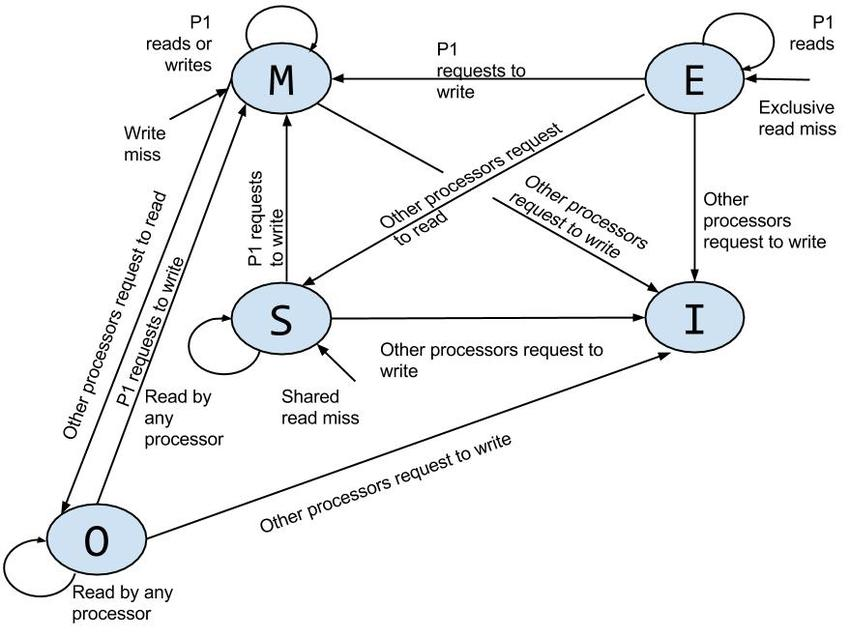
\includegraphics[width=10cm]{images/moesi.png}
    \caption{\label{pic:moesi} Fonctionnement du protocole MOESI (source \cite{Sayin2014})}
\end{figure}





\paragraph{Protocole globaux - Cohérence par répertoire (\textit{directory based coherence}).}

La seconde famille regroupe les protocoles dits \textit{globaux} utilisent des répertoires et des contrôleurs émettant les commandes de transferts des lignes de cache (entre les caches ou avec la mémoire)\cite{tang1976cache}. Toutes les informations nécessaires à la gestion de la cohérence sont enregistrées dans un répertoire. Leur performance est meilleure que les protocoles utilisant des techniques de \textit{snooping} et \textit{broadcasting} car ils génèrent moins de trafic. Bien que les protocoles tels que MOESI réduisent le trafic mémoire en utilisant des écritures différées, la gestion des cinq états est complexe. Et le trafic généré par la cohérence de cache augmente fortement avec le nombre de coeurs utilisés et peu rapidement voir ses performances s'effondrer \cite{liu2016protocoles}. Les futures architectures à mémoire partagée nécessiteront d'implémenter des protocoles de cohérence de cache très performant  \cite{al2010snoopy}.





%%%%%%%%%%%%%%%%%%%%%%%%%%%%%%%%%%%%%%%%%%%%%%%%%%%%%%%%%%%%%%%%%%%
%%%%%%%%%%%%%%%%%%%%%%%%%%%%%%%%%%%%%%%%%%%%%%%%%%%%%%%%%%%%%%%%%%%
